\documentclass[a4paper]{report}
\usepackage[textwidth=17cm, textheight=25cm]{geometry}
\usepackage{verbatim}

\usepackage[utf8]{inputenc}
\usepackage[ngerman]{babel}
\usepackage[pdftex]{hyperref}
\usepackage{framed}
\usepackage{mdframed}

\usepackage{amsmath, amssymb}
\usepackage{enumerate}
\usepackage{multicol} % multiple collums in enumerate
\usepackage{graphicx}
\usepackage{tabu}
\title{C++ in Übersichten \\ \medskip \large Material zum C++ Kurs}
\author{Maximilian Starke \\ Student der TU Dresden \\ Fakultät Informatik}
\date{\today}

%\usepackage[thmmarks,amsmath,hyperref,noconfig]{ntheorem}
\usepackage{listings}
\usepackage{fancybox}
\input{syntax.tex}
\usepackage{tikz}
\usepackage{rail}
\usepackage{struktex}
% RAIL INIT
\railalias{raildollar}{\$}
\railalias{raillbrace}{\textrm{\{}}
\railalias{railrbrace}{\textrm{\}}}
\railterm{raildollar, raillbrace, railrbrace}

\usepackage{array}
\newcolumntype{P}[1]{>{\centering\arraybackslash}p{#1}}
\newcolumntype{M}[1]{>{\centering\arraybackslash}m{#1}}


\usepackage{tikz}
\usetikzlibrary{shapes,arrows}


\usetikzlibrary{%
	arrows,%
	shapes.misc,% wg. rounded rectangle
	shapes.arrows,%
	chains,%
	matrix,%
	positioning,% wg. " of "
	scopes,%
	decorations.pathmorphing,% /pgf/decoration/random steps | erste Graphik
	shadows%
}


\usepackage{caption}
\DeclareCaptionFont{white}{\color{white}}

\lstset{language=C++}
\usepackage{xcolor}
\usepackage{listings}
\usepackage{tcolorbox}
\tcbuselibrary{listings}
%\usepackage{minted}
%\tcbuselibrary{minted}
% maybe install minted some day and make syntax highlighting###

\begin{document}

\maketitle

\section*{Vorwort}
Dieses Skript \textbf{C++ in Übersichten} enthält Material zum C++ Kurs, den ich im Sommersemester 2017 halte (\url{ifsr.de/kurse})
Das Skript wird parallel zum Kurs erstellt und erweitert. Es besteht daher momentan noch als Entwurf.

Das Skript dient vordergründig als Nachschlagewerk für den C++ Kurs und besteht im Wesentlichen aus vier Kapiteln zu Einrichtung, Datentypen, strukturierter Programmierung und Randfeatures. Dabei wurde in erster Linie eine Einteilung nach logischen Zusammenhängen der Sprache C++ angestrebt, zweitrangig nach pädagogisch sinnvoller Reihenfolge. Das stellt mehr oder weniger eine hinreichende und zugleich notwendige Bedingung für die parallele Abarbeitung von Kapitel 2 und 3 dar, da Kenntnisse über Datentypen und Mechanismen strukturierter Programmierung an vielen Stellen wieder eine Einheit bilden und ineinander greifen.

\tableofcontents

\chapter{Einrichtung}

\section{ISO C++}

\subsection{Allgemeines}
\begin{itemize}
\item ab 1979 von Bjarne Stroustrup bei AT\&T entwickelt als Erweiterung der Programmiersprache C
\item später von ISO genormt
\vspace{2ex}
\item effizient und schnell - Schnelligkeit eines der wichtigsten Designprinzipien von C++
\item hohes Abstraktionsniveau u.a. durch Unterstützung von OOP
\item ISO Standard beschreibt auch eine Standardbibliothek
\item C++ ist \textbf{kein} echtes \textit{(und auch kein unechtes)} Superset von C (siehe stackoverflow.com, \dots)
\item C++ ist (wie C) \textbf{case sensitive}
\vspace{2ex}

\item Paradigmen:
	\begin{itemize}
		\item \textbf{generisch} (durch Benutzung von Templates, automatische Erstellung multipler Funktionen für verschiedene Datentypen)
		\item \textbf{imperativ} (Programm als Folge von Anweisungen, Gegenteil von deklarativ siehe Haskell und Logikprogrammierung)
		\item \textbf{objektorientiert} (Klassen, Objekte, Vererbung, Polymorphie, Idee: Anlehnung an Realität)
		\item \textbf{prozedural} (Begriff mit verschiedenen Bedeutungsauffassungen, Unterteilung des Programms in logische Teilstücke (Prozeduren), die bestimmte Aufgaben / Funktionen übernehmen)
		\item \textbf{strukturiert} (prozedural und Teilung in Sequenz, Verzweigung, Wiederholung, \dots )
		\item \textbf{funktional} (ab C++11, Definitionskleinkram, siehe Wikipedia, Programm als verschachtelter [...] Funktionsaufruf 	organisierbar, eher typisch für Haskell o.ä.)
	\end{itemize}
\end{itemize}

\subsection{Versionen}
\begin{itemize}
	\item C++98
	\item C++03
	\item C++11
	\subitem wesentliche Neuerungen. Einführung von constexpr, Elementinitialisierer, ... Neue Bedeutung des Schlüsselworts auto \hspace{3cm} \# Referenzen ergänzen %#####
	\item C++14
	\subitem aufweichung der constexpr Bedingungen.
	\item C++17
	\subitem soll 2017 vollendet werden.
\end{itemize}

\section{Dateien in einem C++ Projekt}
\begin{center}
\begin{tabular}{|c|c|p{8.5cm}|}
	\hline
	Dateiendung & Bezeichnung & Inhalt \\
	\hline
	(*.cpp) (*.cc) & Quelldatei & Funktionsimplementation, Klassenimplementation, \newline Berechnungen bzw. eigentliche Arbeit erledigen \\ \hline
	(*.h) & Headerdatei & Funktionsdeklaration, Klassendefinition, \newline Bezeichner öffentlich bekannt machen \\
	\hline
	(*.o) & Objektdatei & Objektcode (Maschinencode) einer Übersetzungseinheit\\
	\hline
	(*.exe) (*.out) & ausführbare Datei & fertiges Programm \\
	\hline \hline
	(*.sln) (*.pro) (*.vcxproj) & "Projektdatei" & IDE Einstellungen (oder ähnliches) \newline IDE-spezifische Namen und Verwendung\\
	\hline \hline
	(*.res) & Ressourcendatei & multimediale Inhalte\\
	\hline
\end{tabular}

\vspace{4ex}

% Define block styles
\tikzstyle{block} = [rectangle, draw, fill=blue!40, 
text width=7em, text centered, rounded corners, minimum height=5em, node distance= 4.5cm, line width = 2pt]


\tikzstyle{cblock} = [rectangle, draw, fill=blue!40, 
text width=7em, text centered, rounded corners, minimum height=5em, node distance= 3.0cm, line width = 2pt]


\tikzstyle{line} = [draw, -latex', line width = 4pt]


\tikzstyle{cloud} = [draw, ellipse,fill=red!40, node distance=3cm, line width = 2pt,
minimum height=3em]

{\large

\begin{tikzpicture}[node distance = 3cm, auto]
    % Place nodes
    \node [cloud] (pc) {Precompiler};
    
    \node [block, left of=pc] (cpp) {*cpp, *.c};
    \path [line] (cpp) --(pc);
    
    \node [block, right of=pc] (h) {*.h};
    \path [line] (h) --(pc);
    
    \node [cblock, below of=pc] (cpp2) {cpp without \#precompiler instruction};
    \path [line, below of = cpp2] (pc) -- (cpp2);
    
    \node [cloud, below of = cpp2] (c) {Compiler};
    \path [line] (cpp2) -- (c);
    
    \node [cblock, below of = c] (o) {*.o};
    \path [line] (c) -- (o);
    
    \node [cloud, below of = o] (l) {Linker};
    \path [line] (o) -- (l);
    
    \node [block, left of =o] (lo) {another\\ *.o};
    \path [line] (lo) -- (l);
    
    \node [block, right of = o] (ro) {another\\ *.o};
    \path [line] (ro) -- (l);
    
    \node [cblock, below of = l] (exe) {*.exe, *.out};
    \path [line] (l) -- (exe);
     
    \node [block, right of = exe] (lib) {*.lib, *.dll};
    \path [line] (l) -- (lib); 

\end{tikzpicture}
}
\end{center}


\section{Compiler}
\begin{center}
\begin{tabular}{|c|l|}
	\hline
	\textbf{Compiler} & \textbf{Plattform} \\ \hline \hline
	GCC/g++ & Windows, Linux, Mac, Unix-like \\ \hline
	Clang & Unix-like, Mac, Windows, Linux \\ \hline
	Intel-C++ & Linux, Windows, Mac \\ \hline
	VC++ & Windows \\ \hline
\end{tabular}
\end{center}
Das nun folgende Listing zeigt, wie ein C++ Quellcode, der als Datei vorliegt, "`per Hand"' mit Kommandozeile unter Nutzung des Compilers (hier g++) übersetzt werden kann. Beim Aufruf des Compilers wurden hier noch einige Flags gesetzt, nämlich \texttt{-Wall}, um \textbf{sinnvolle Warnungen} ausgeben zu lassen, und \texttt{-pedantic}, um \textbf{vom C++ Standard geforderte Warnungen} erscheinen zu lassen. Außerdem wurde der C++ Standard (Version) gesetzt.

\begin{tcblisting}{colback=yellow!10,colframe=yellow!40!black,listing only,
		title=Nutzung von g++ mittels Powershell, fonttitle=\bfseries}
PS A:\> cd .\example\
PS A:\example> ls


Verzeichnis: A:\example


Mode                LastWriteTime         Length Name
----                -------------         ------ ----
-a----       02.04.2017     08:38             87 hello_world.cpp


PS A:\example> type .\hello_world.cpp
#include <iostream>

int main(){
	std::cout << "Hello World";
	return 0;
}

PS A:\example> g++ -o programm hello_world.cpp -Wall -pedantic -Wextra -std=c++14
PS A:\example> ls


Verzeichnis: A:\example


Mode                LastWriteTime         Length Name
----                -------------         ------ ----
-a----       02.04.2017     08:38             87 hello_world.cpp
-a----       02.04.2017     09:12          48650 programm.exe


PS A:\example> .\programm.exe
Hello World
PS A:\example>
\end{tcblisting}
%% anmerkung zu Wextra##

Eine kleine Anmerkung zu Bezeichnungen, die mit Compilern zu tun haben, möchte ich an dieser Stelle noch loswerden, da hier immer eine kleine Verwechslungsgefahr besteht. Die \textbf{GCC} \textit{(GNU Compiler Collection)} ist eine Compilersammlung mit Compilern zu C, C++ und einigen weiteren. Dagegen ist der \textbf{gcc} (klein geschrieben) der C-Compiler der Sammlung und \textbf{g++} der C++ Compiler.

Um auf Ihrem Betriebssystem einen C++ Compiler zum Laufen zu bringen, haben Sie meist verschiedenste Möglichkeiten.

Um unter \textbf{Linux} GCC zu nutzen, müssen lediglich die entsprechenden Pakete installiert werden, meist ist die GCC sogar schon vorinstalliert.

Unter \textbf{Windows} kann man den von Microsoft bereitgestellten Visual C++ Compiler verwenden, i.d.R. in Verbindung mit einer Installation von Visual Studio (eine IDE für u.a. C++). Die zu installierenden Komponenten bei Visual Studio kann man selbst beim Installationsprozess auswählen, i.A. ist der Speicherverbrauch jedoch relativ groß. Wer auf eine speicherschonende Variante zurückgreifen will oder muss, dem empfehle ich MinGW - eine Portierung der GCC aus dem Hause Linux für Windows. Planen Sie früher oder später Qt-Creator als eine C++ IDE zu installieren, dann können Sie sich einen extra Installation von MinGW im Vorhinein sparen, da QT-Creator MinGW bereits mitinstalliert. Sofern mit der Kommandozeile direkt auf g++ zugegriffen werden soll, ist es unter Windows i.d.R. erforderlich den Pfad der MinGW-Binarys der Systemvariablen \texttt{PATH} hinzuzufügen.

\begin{comment}
\lstdefinestyle{framed}
{
frame=lrb,        
belowcaptionskip=-1pt,
xleftmargin=8pt,
framexleftmargin=7pt,
framexrightmargin=6pt,
framextopmargin=5pt,
framexbottommargin=5pt,
framesep=0pt,
rulesep=0pt,
}

\begin{lstlisting}[style = framed, caption = Nutzung von g++ mittels Powershell]
PS A:\> cd .\example\
PS A:\example> ls


Verzeichnis: A:\example


Mode                LastWriteTime         Length Name
----                -------------         ------ ----
-a----       02.04.2017     08:38             87 hello_world.cpp


PS A:\example> type .\hello_world.cpp
#include <iostream>

int main(){
	std::cout << "Hello World";
	return 0;
}
	
PS A:\example> g++ -o programm hello_world.cpp -Wall -pedantic -std=c++11
PS A:\example> ls


Verzeichnis: A:\example


Mode                LastWriteTime         Length Name
----                -------------         ------ ----
-a----       02.04.2017     08:38             87 hello_world.cpp
-a----       02.04.2017     09:12          48650 programm.exe


PS A:\example> .\programm.exe
Hello World
PS A:\example>
\end{lstlisting}
\end{comment}


\section{IDEs}
\subsection{JA oder NEIN}
\begin{center}
\begin{tabular}{|c||c|}
	\hline
	\textbf{ohne IDE} & \textbf{mit IDE} \\
	\hline \hline
	Compiler, Linker über Shell bedienen	&	Projekteinstellungen \& Buttons \\
	Texteditor				&		in IDE integriert\\
	evtl. make + makefile	&	automatisch generiertes makefile \\
	Dokumentationen & geordneter Menübaum \\
	\hline \hline
	Einarbeitungszeit (??) & Einarbeitungszeit (??) \\
	für kleine und mittelgroße Projekte & kleine, mittlere und große Projekte \\
	\hline
\end{tabular}
\end{center}

\subsection{IDEs im Überblick}
\begin{center}
\begin{tabular}{|c|c|p{10cm}|}
	\hline
	\textbf{IDE} & \textbf{Plattform} & \textbf{Anmerkungen}\\
	\hline
	Eclipse, Netbeans & Java (JVM) & in und für Java geschrieben, unterstützt auch C++ \\
	Qt SDK & WIN, Linux, Mac & bringt umfangreiches Qt-Framework mit für GUIs u.v.m. \\
	Code::Blocks & WIN, Linux, Mac & \\
	\hline
	Visual Studio & Windows & kostenfreie Version für den Hausgebrauch: VS Community 2017, sehr umfangreich (Refactoring Tools, Debugger, Laufzeitanalyse, Frameworks wie MFC, ATL, WTL) und damit auch speicherintensiv, zu installierende Features wählbar, benutzt eigenen MS VC++ Compiler\\
	Orwell DEV-C++ & Windows &\\
	\hline
	Geany & Linux, WIN & schlichter Texteditor mit Syntaxhighlighting und diversen Buttons für Compilerausführung, Logausgabe\\
	KDevelop & Linux, WIN & \# \\ %#####
	Anjuta & Linux & \# \\ %#####
	\hline
	XCode & MacOS & "`hauseigene"' IDE von Apple\\
	\hline
	
\end{tabular}

\vspace{4ex}

Auf den Seiten \pageref{begin:ide:picts} bis \pageref{end:ide:picts} finden sich Screenshots einiger IDEs.

\begin{figure}
	\label{begin:ide:picts}
	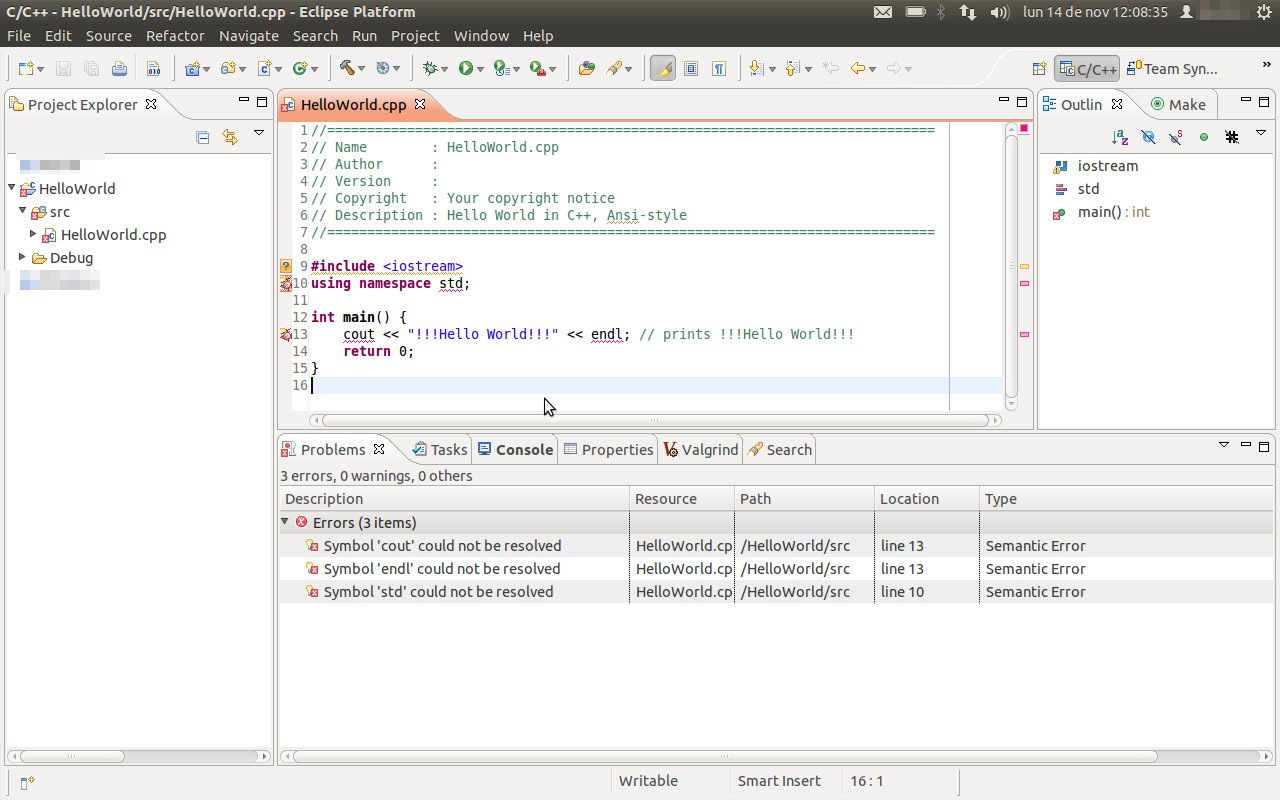
\includegraphics[width = \textwidth]{01/eclipse.jpg}
	\caption{Eclipse mit einem C++ Projekt}
	\url{https://www.eclipse.org/forums/index.php/fa/6135/0/}
	\label{pic:eclipse}
\end{figure}
\begin{figure}
	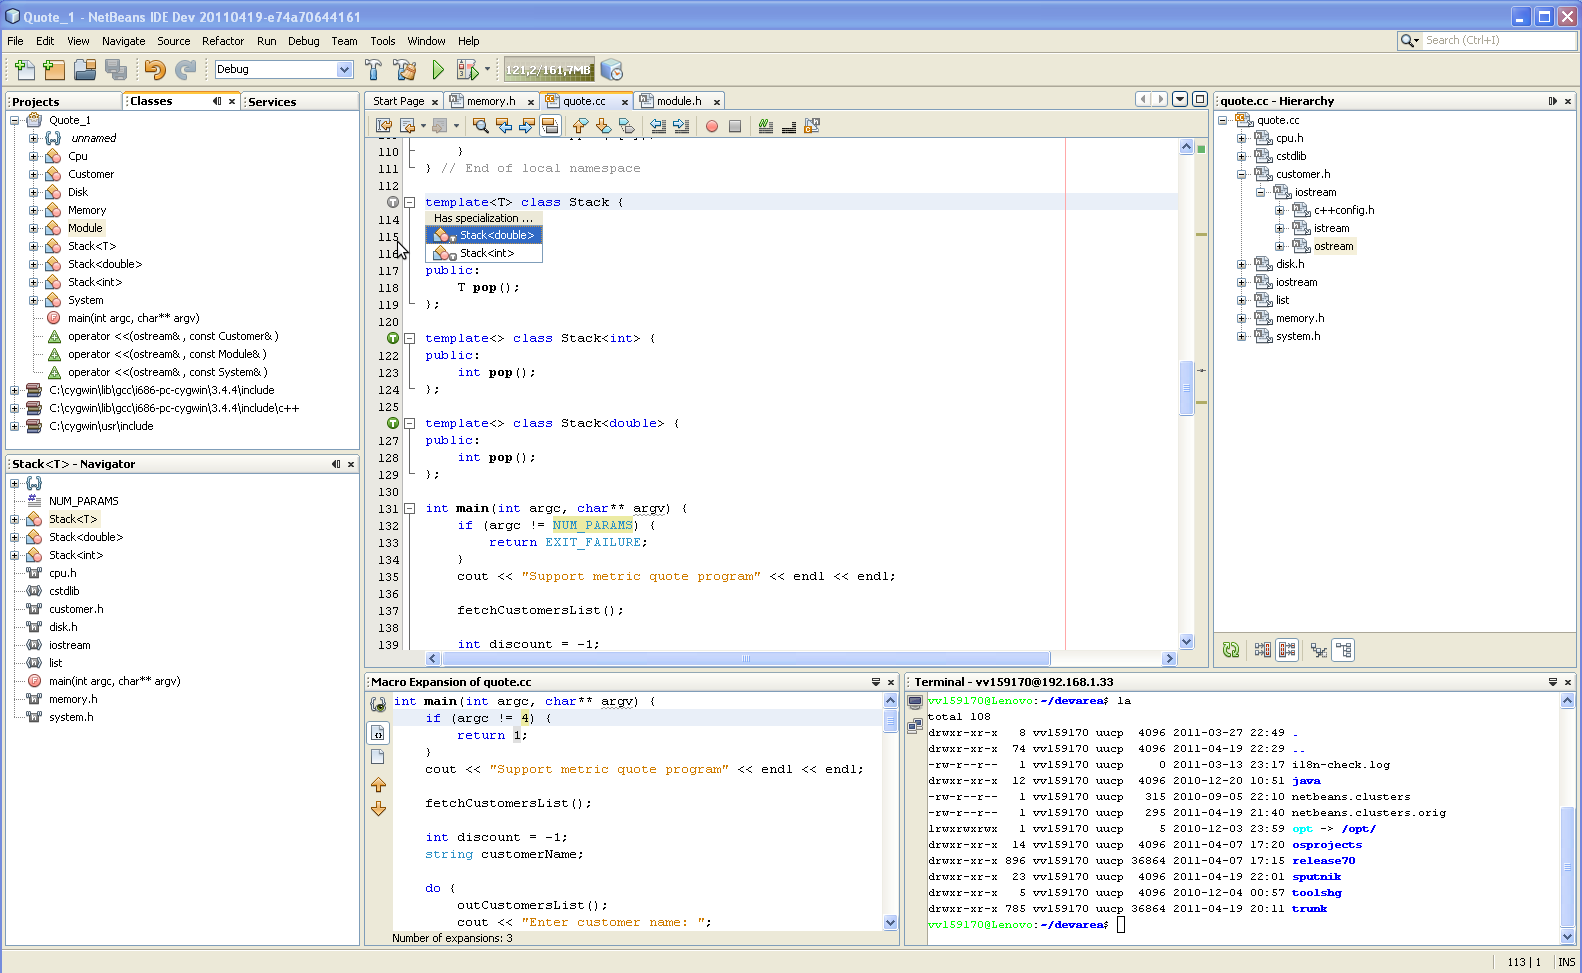
\includegraphics[width = \textwidth]{01/netbeans.png}
	\caption{NetBeans und die Verwendung von C++}
	\url{https://netbeans.org/images_www/v7/screenshots/cnd.png}
	\label{pic:netbeans}
\end{figure}
\begin{figure}
	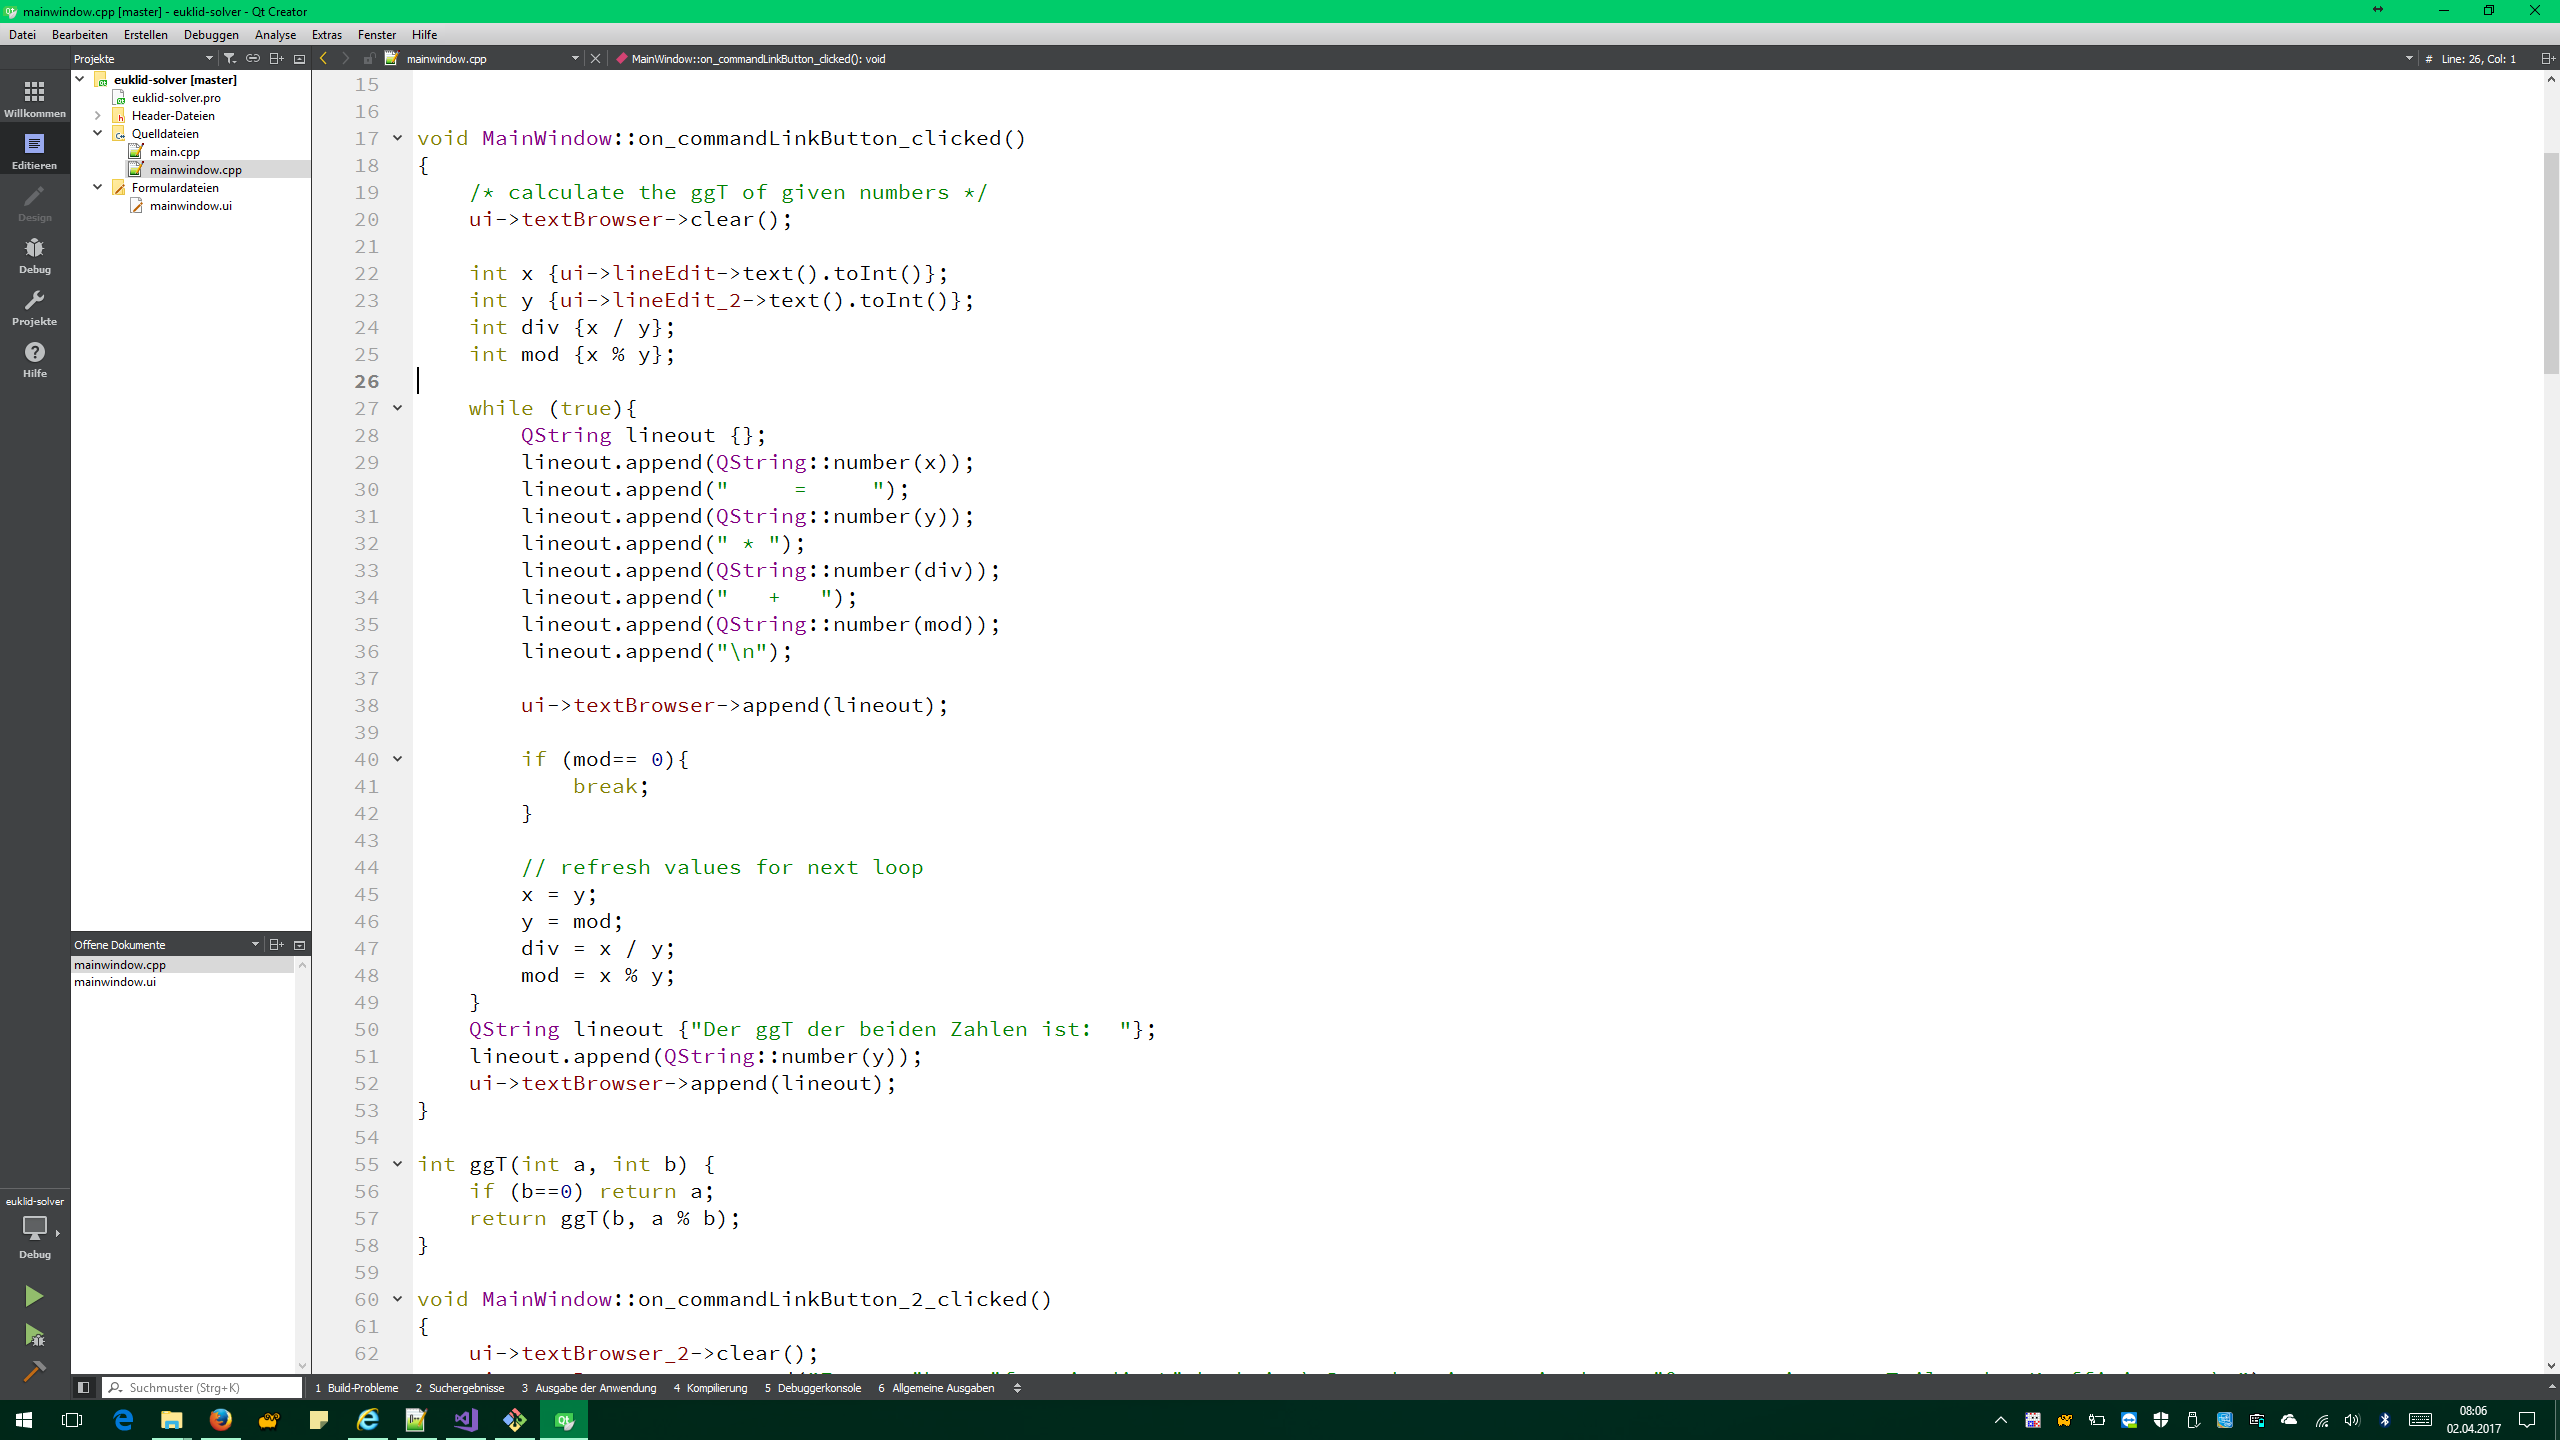
\includegraphics[width = \textwidth]{01/qt_code.png}
	\caption{C++ Code in der QT Creator IDE}
	\label{pic:qt_code}
\end{figure}
\begin{figure}
	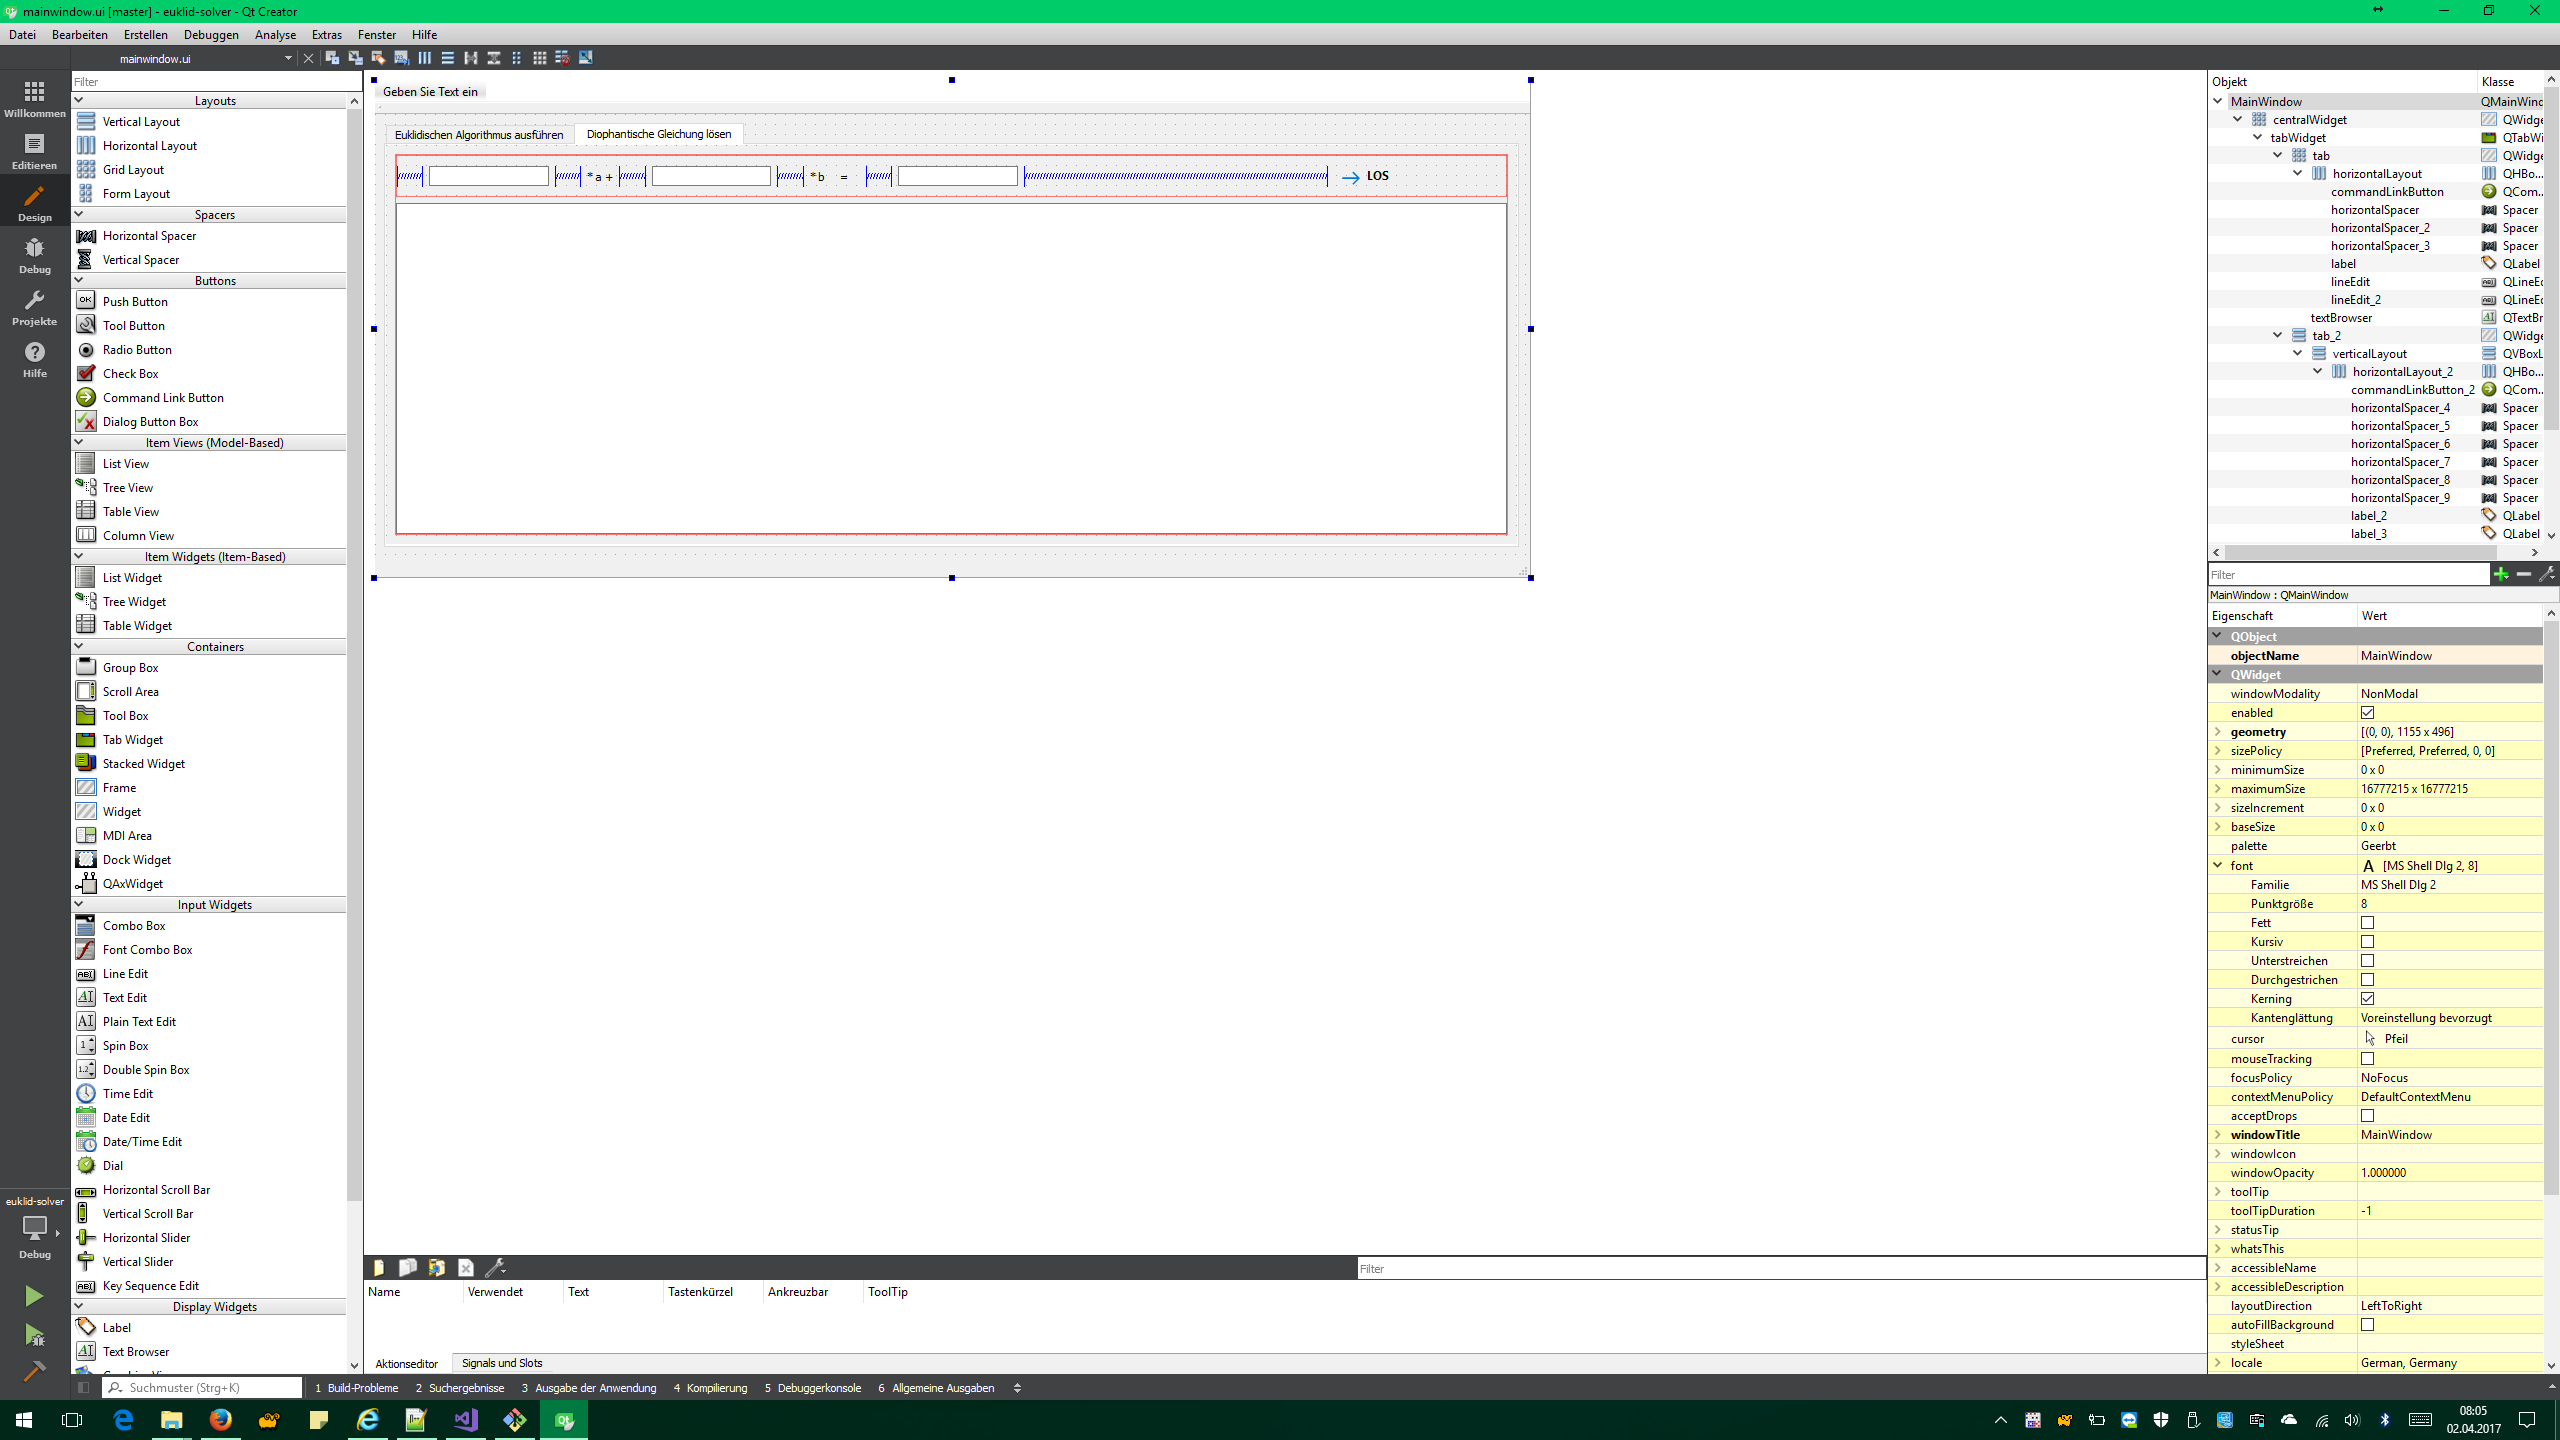
\includegraphics[width = \textwidth]{01/qt_designer.png}
	\caption{Fensterdesign mit QT Creator}
	\label{pic:qt_designer}
\end{figure}
\begin{figure}
	\centering
	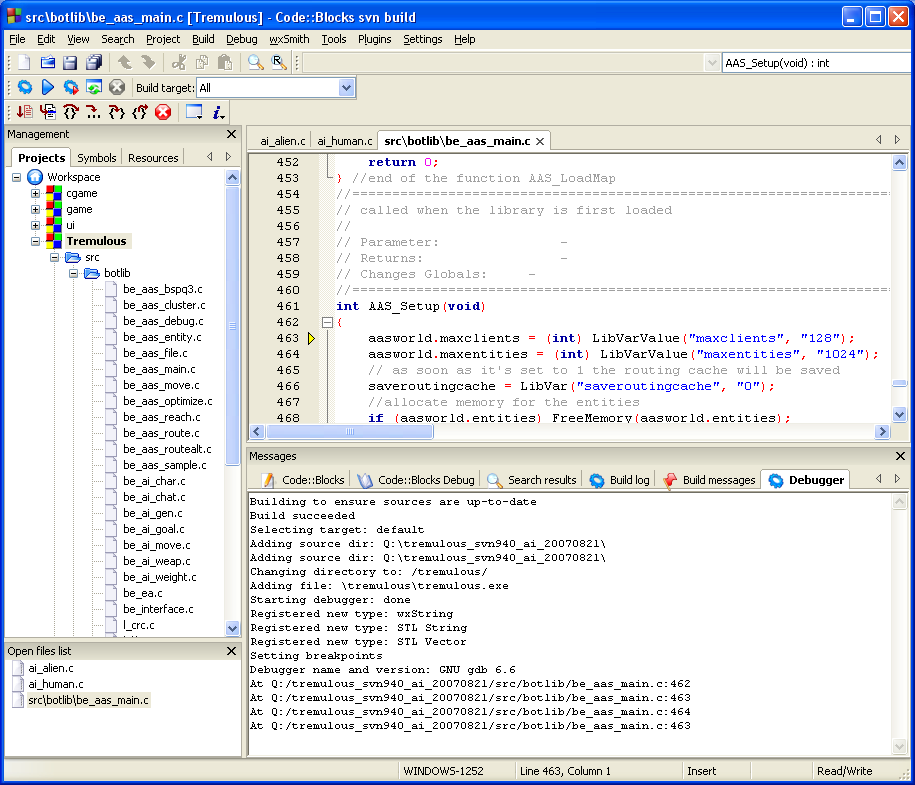
\includegraphics[width = 13cm]{01/codeblocks.png}
	\caption{Code Blocks}
	\label{pic:code::blocks}
	\url{http://www.aftermoon.net/img/20070905_codeblocks_tremulous.png}
\end{figure}
\begin{figure}
	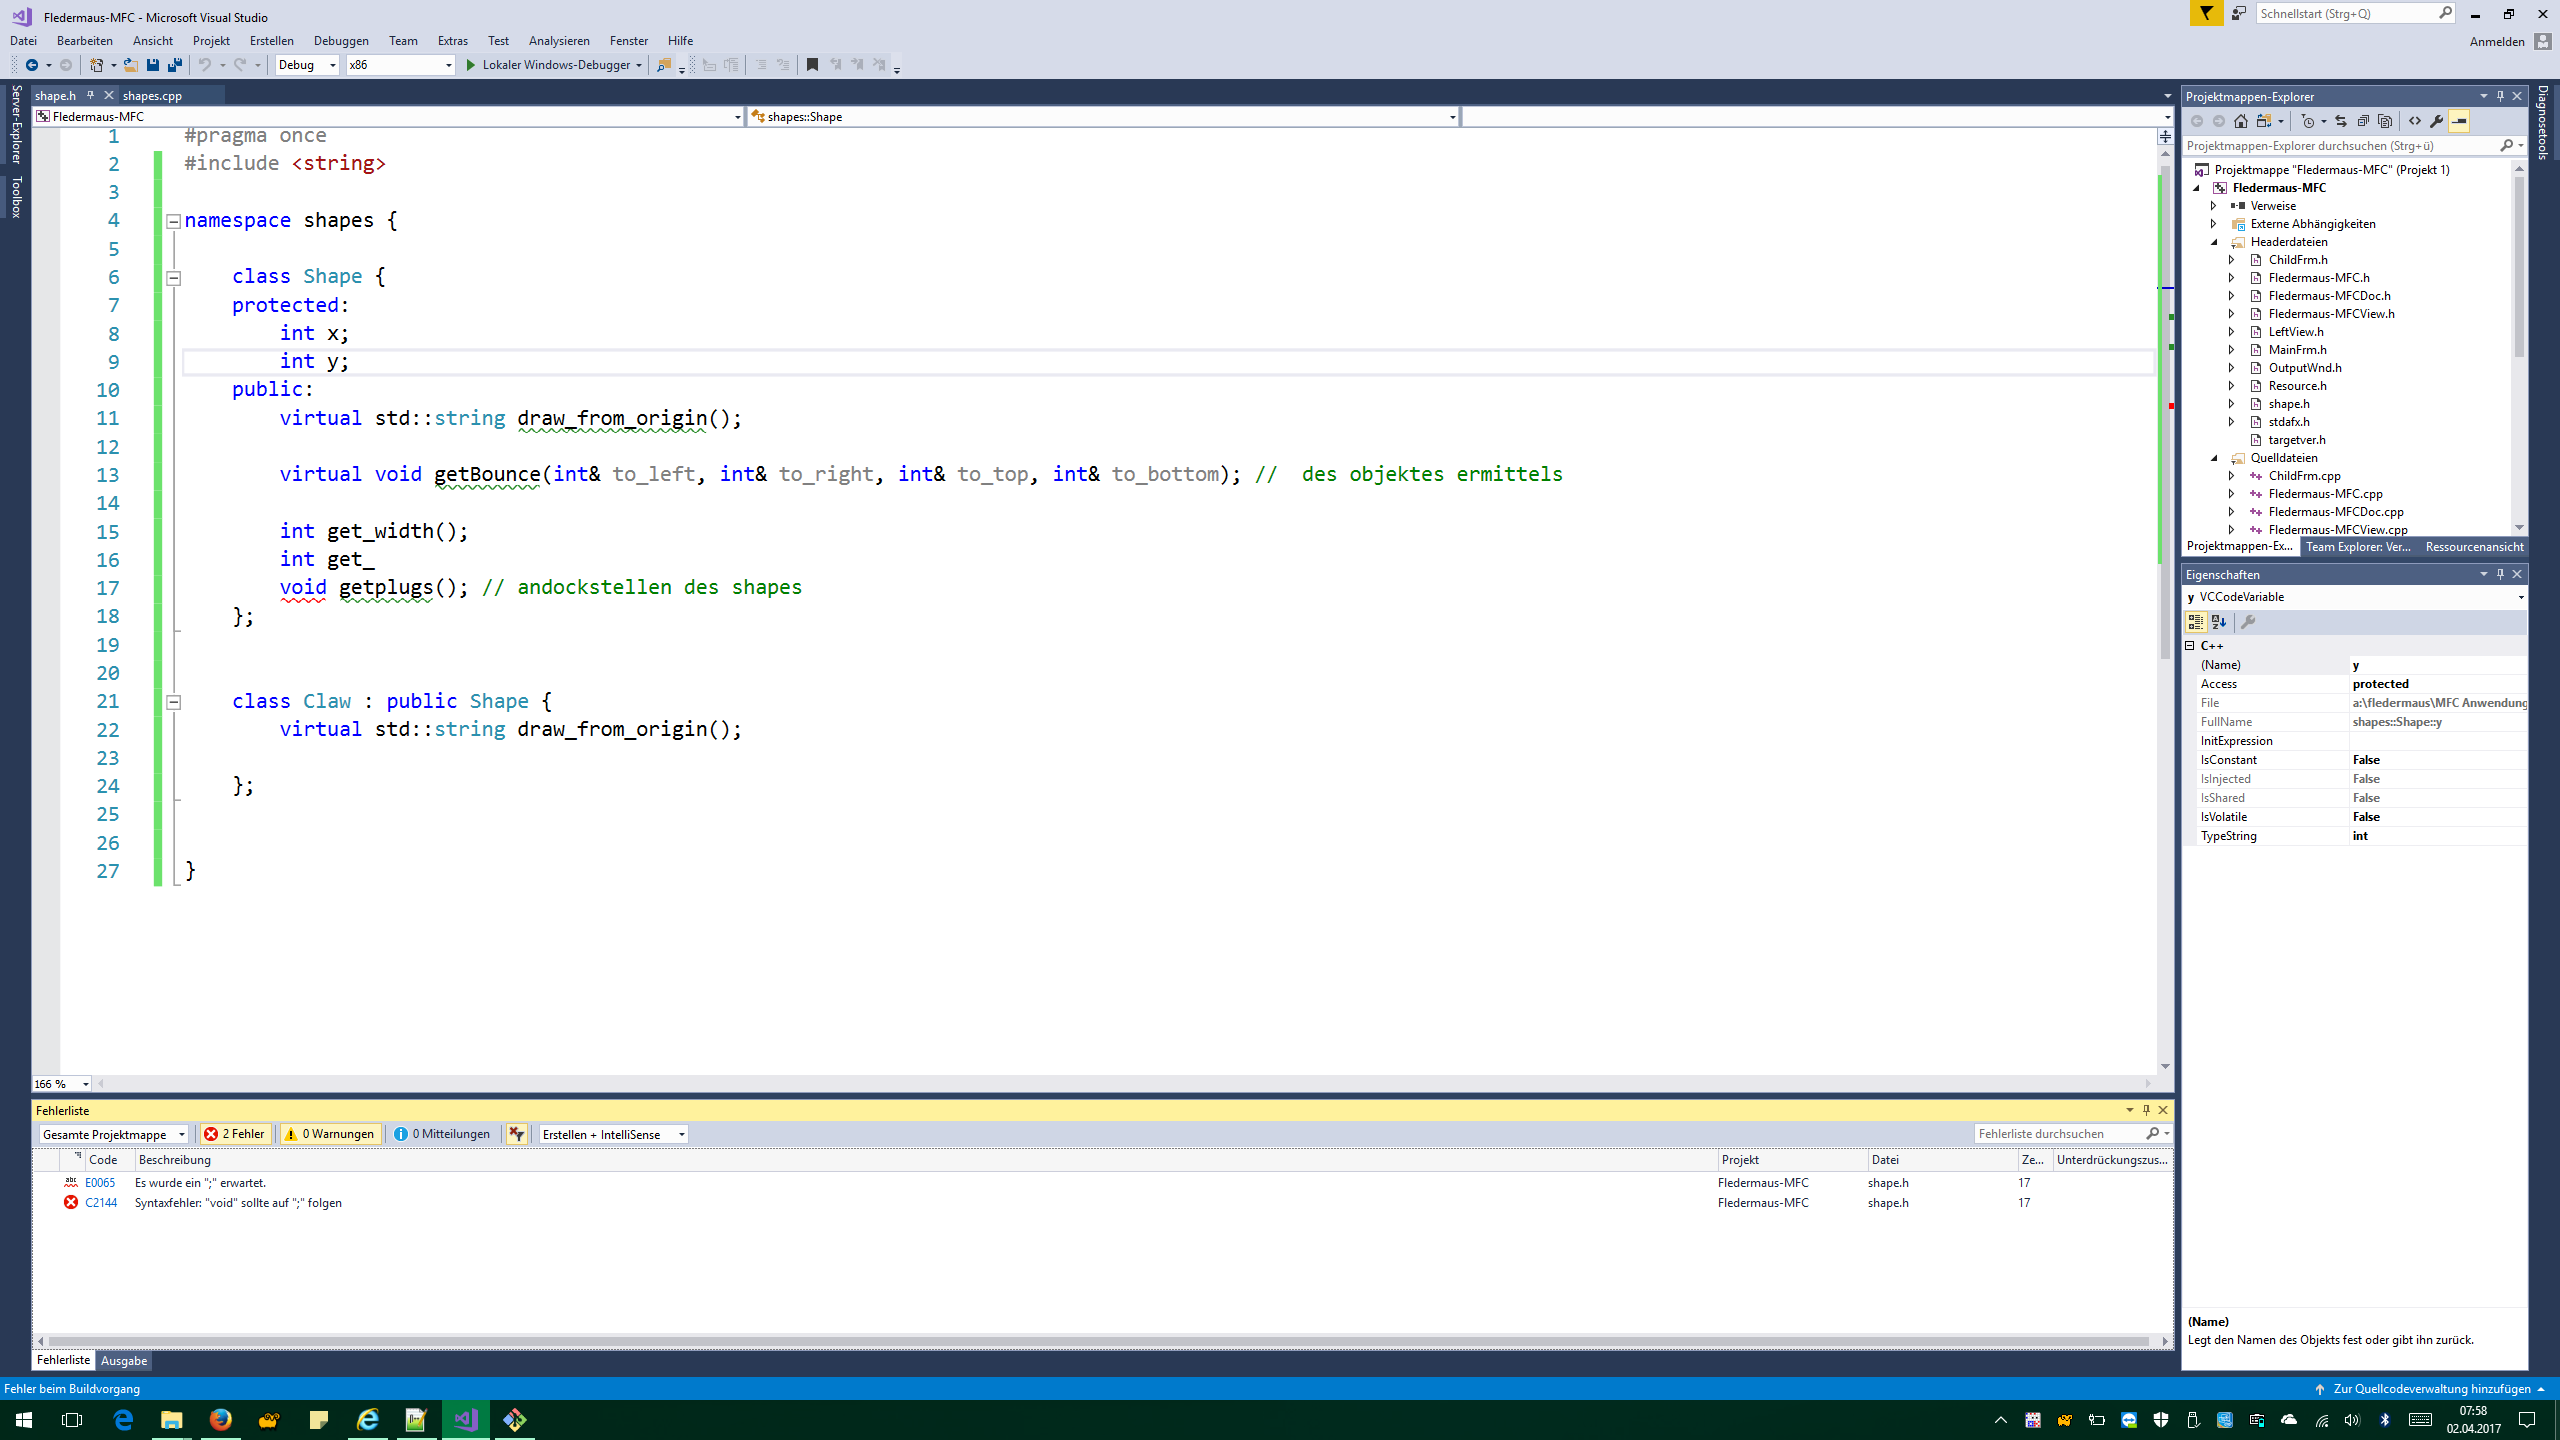
\includegraphics[width = \textwidth]{01/vs.png}
	\caption{Visual Studio Community}
	\label{pic:visualstudio}	
\end{figure}
\begin{figure}
	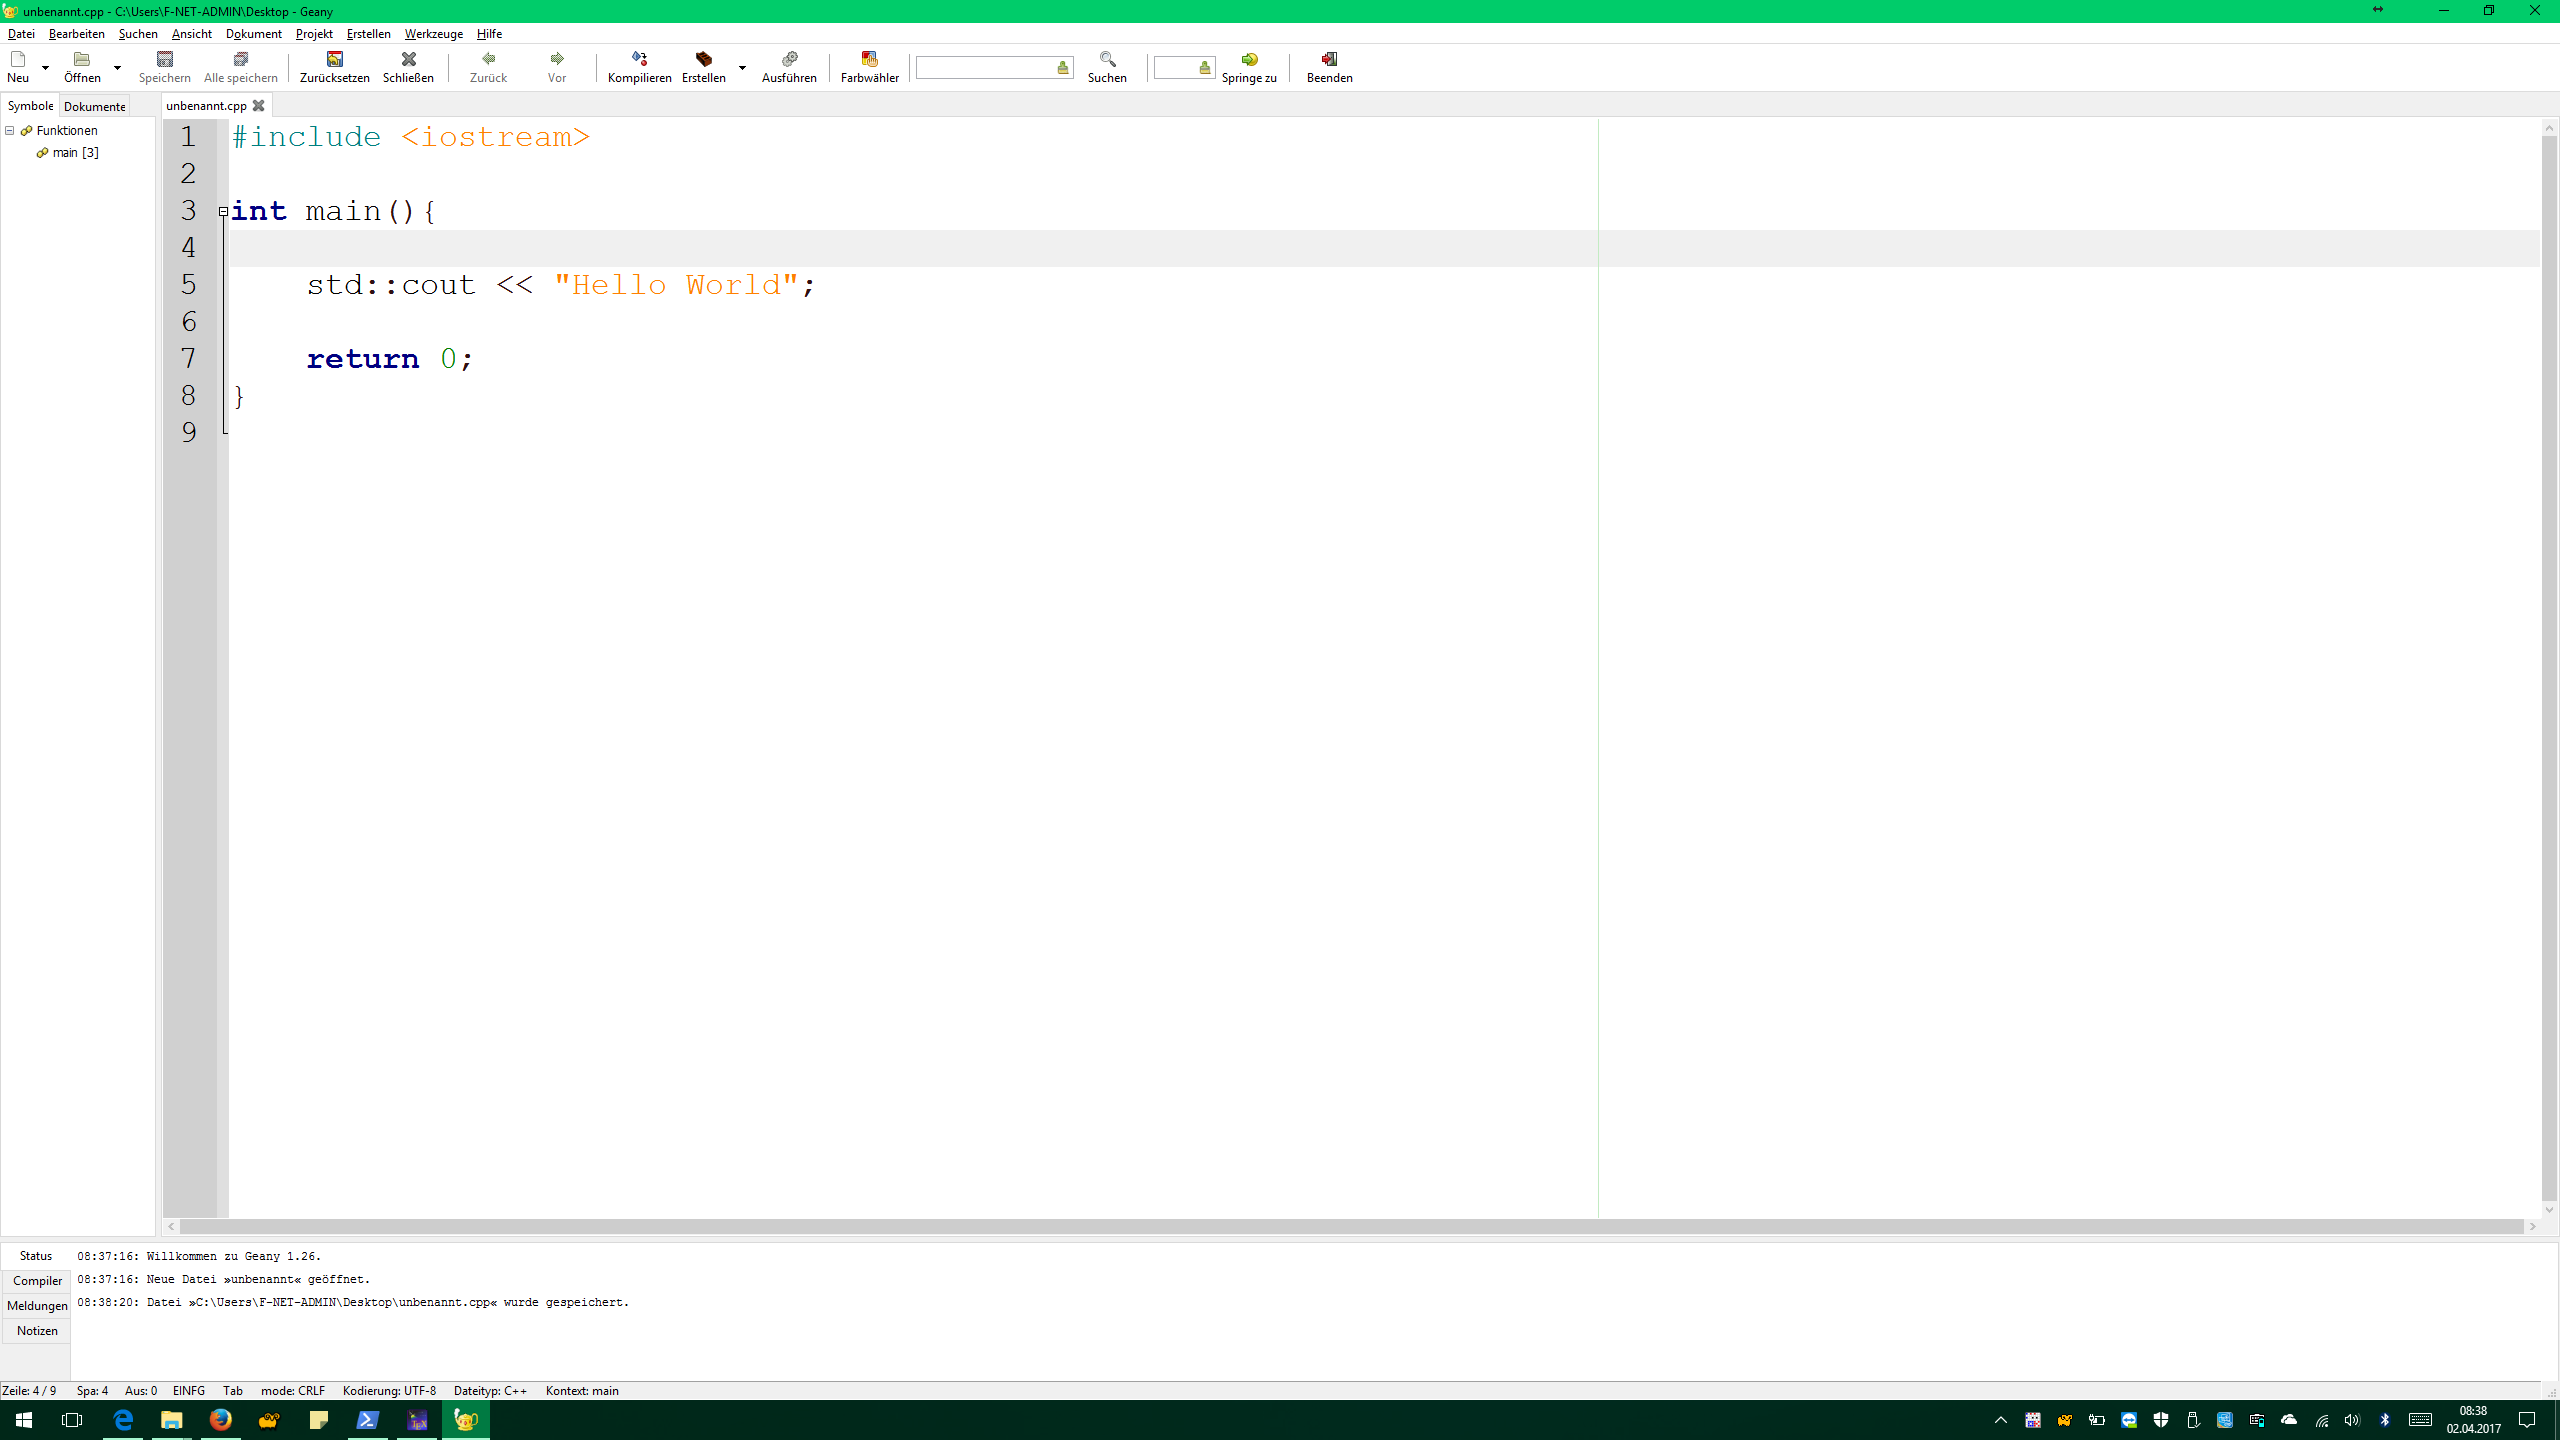
\includegraphics[width = \textwidth]{01/geany.png}
	\caption{Geany}
	\label{pic:geany}	
\end{figure}
\begin{figure}
	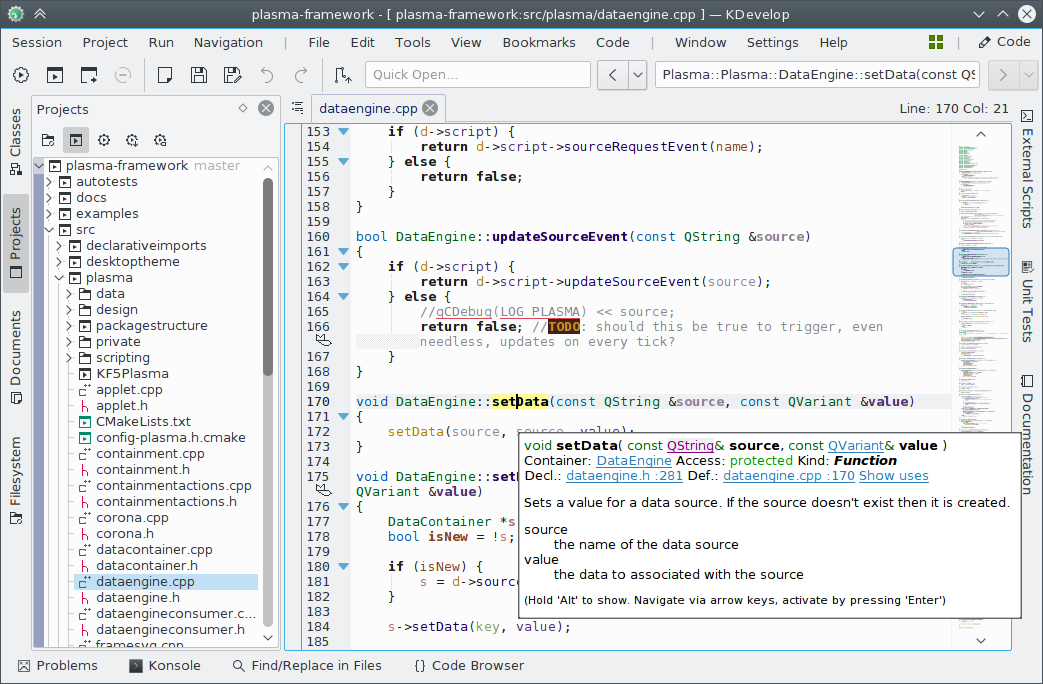
\includegraphics[width = \textwidth]{01/kdevelop.png}
	\caption{KDevelop}
	\url{https://www.kdevelop.org/sites/www.kdevelop.org/files/inline-images/kdevelop5-breeze_2.png}
	\label{pic:kdevelop}	
	\label{end:ide:picts}
\end{figure}
\end{center}

\section{Referenzen}

\begin{itemize}
	\item Buch:
	\begin{itemize}
		\item Wolf, Jürgen: C++ - Das umfassende Handbuch. Rheinwerk Computing
	\end{itemize}
	\item Websites:
	\begin{itemize}
		\item \url{http://en.cppreference.com/w/}
		\item \url{ttp://www.cplusplus.com/reference/}
	\end{itemize}
\end{itemize}
%\###### Anmerkung ergänzen (Buch)
\# Es gibt auch offline Versionen der Referenzen.
\section{The Hello World}

\subsection{Das erste kleine Programm}
\begin{tcblisting}{colback=yellow!10,colframe=yellow!40!black,listing only,
		title=Unser erstes C++ Programm, fonttitle=\bfseries}
#include <iostream>
// "Einbinden" d.h. 1-zu-1-Einfuegen des Headers iostream.h

int main(int argc, char* argv[])
// main-Funktion: Einstiegspunkt der Anwendung
// count: Anzahl der uebergebenen Parameter 
// arg: Pointer auf ein Array von Pointern auf C-Style-Strings (die Parameter)
// Parameter der main-Funktion duerfen in der Signatur auch weggelassen werden.

// Parameter der main-Funktion 
{   // Beginn vom Anweisungsblock der main-Funktion
	
	std::cout << "Hello World" << std::endl;
	// Ausgabe von "Hello World" und Zeilenumbruch
	// genauer:
	/*
	* implizite Klammerung:
	* ((std::cout) << "Hello World") << (std::endl);
	* std              ... ein Namensraum
	* ::               ... scope-Operator (Bereichsoperator)
	* cout:            ... gepufferter Standardausgabestream
	* <<               ... Ausgabeoperator (auch bitshift-Operator)
	* "Hello World"    ... C-Style-String Literal
	* endl             ... Objekt aus dem std Namensraum, das einen Zeilenumbruch ('\n') erzeugt.
	* ;                ... Abschluss einer einzelnen Anweisung
	*/
	
	for(int i = 0; i < argc; ++i ){
		std::cout << i << ". Parameter:  " << argv[i] << '\n';
	} // Beipiel fuer die Ausgabe der Komandozeilenargumente
	// argv[0] ist der Name der executable Datei
	
	return 0; // Rueckgabewert 0 "erfolgreich (ohne Fehler) beendet"
}
\end{tcblisting}
Im Falle der \texttt{main-}Funktion ist es auch möglich das \textbf{return statement} (\texttt{return 0;}) wegzulassen. Dann wird implizit 0 als Funktionswert zurückgegeben. Die Funktionssignatur der \texttt{main-}Funktion darf auch in \texttt{int main(int argc, char** argv)} geändert werden. Der erste Arrayeintrag von \texttt{argv} enthält übrigens immer einen Zeiger auf den Namen (ohne Dateiendung), unter dem das Programm abgespeichert wurde. Damit ist \texttt{argc} stets mindestens 1. 
\subsection{Ein paar Werkzeuge}
Bevor wir in Kapitel \ref{real_start} einsteigen und das gesamte (naja \textit{fast}) C++ von Grund auf kennenlernen wollen, sollten Sie noch einige nützliche Werkzeuge kennen, damit Sie neu gelernte Dinge auch ohne große Probleme ausprobieren können.
\begin{tcblisting}{colback=yellow!10,colframe=yellow!40!black,listing only,
		title=... und ein paar Hilfsmittel ..., fonttitle=\bfseries}
#include <iostream>


#define debug // Benutzung bedingter Compilierung zum Debugging

int main(int argc, char* argv[]){
	
	int zahl = 0;
	std::cout << "Wie alt bist du?\n"; // eine simple Ausgabe
	std::cin >> zahl; // eine simple Eingabe
	std::cout << "Okay!\n\n";
	
#ifndef debug 
	//folgende Zeile compiliert nicht:
	std::cout << << "In 7 Jahren bist du " << 7 + zahl << " Jahre alt." << '\n';
#endif //debug
	
	std::cout << "Tsch" << static_cast<char>(0x81) << "ss\n";
	//https://de.wikipedia.org/wiki/Codepage_850
	
	std::cin.sync();
	std::cin.get(); // warted auf Enter zum fortfahren.
	
	/*
	Das ist
	ein mehrzeiliger
	Kommentar
	*/
	
	// Das ist ein einzeiliger Kommentar.
}
\end{tcblisting}
\begin{center}
\begin{tabular}{|c|c|}
	\hline
	\textbf{Objekt} & \textbf{Funktionalität} \\
	\hline \hline
	\texttt{cin}	& Standardeingabe, standardmäßig Eingabe von Tastatur \\
	\hline
	\texttt{cout}	& (gepufferte) Standardausgabe \\
	\texttt{cerr}	& ungepufferte Standardfehlerausgabe \\
	\texttt{clog}	& gepufferte Standardfehlerausgabe \\
	\hline
	\multicolumn{2}{|p{11cm}|}{\textbf{Achtung: Diese Streamobjekte liegen alle im Namensraum \texttt{std} und werden nach einem \texttt{\#include <iostream>} erst verfügbar}}\\
	\hline
\end{tabular}
\end{center}

\subsection{Programmierstil}
Bevor es richtig losgeht, möchte ich noch ein paar Worte über den Programmierstil loswerden. Im Grunde genommen dürfen Sie Ihren C++ Code schreiben, wie sie wollen, solange Sie die Spezifikationen von c++ einhalten. Es gibt auch nicht \textit{den einen} Programmierstil, der sich durchgesetzt hat. Sie schreiben aber einen viel leserlicheren, einfacher wartbaren und für das Auge schöneren Code, wenn Sie beim programmieren \textbf{konsistent bleiben}, was einige Aspekte betrifft:
\begin{center}
	\begin{tabular}{|c||c|}
		\hline
		Einrückungen	&	tabs or spaces \\ \hline
		Anweisungen pro Zeile & eine, ... \\ \hline
		Bezeichner		&	snake\_case, camelCase, PascalCase \\
		& kurz, prägnant, aussagekräftig \\ 
		& Deutsch, Englisch, \dots Isländisch \\ \hline
	\end{tabular}
\end{center}
Einige IDEs können Sie sogar mehr oder weniger dabei unterstützen, in dem Sie sich um die \textbf{Quelltextformatierung} kümmern. Dies ist gerade bei Projekten mit vielen Entwicklern hilfreich, da so ziemlich effizient für einheitliches Quelltextlayout gesorgt werden kann.

\begin{comment}
	Inhalt...
\end{comment}
\chapter{Datentypen in C++} \label{real_start}

Früher oder später müssen Sie in Ihrem Programm Daten speichern, sei es während der Laufzeit im Arbeitsspeicher (RAM) oder darüber hinaus persistent in Dateien, die Sie in Dateisystemen auf zum Beispiel Festplatten aufbewahren können. Dabei steht in der Regel als erstes die \textbf{Wahl des Datentypes} im Vordergrund, denn die Wahl des Datentyps bestimmt maßgeblich die \textbf{Möglichkeiten der Verwendung der Daten}. So gibt Ihnen der Datentyp grundsätzlich vor welche Funktionen und insbesondere Operatoren Sie darauf anwenden können, beziehungsweise \textit{was} diese bewirken.

\section{Identifier}
%\begin{comment}%debug


\begin{multicols}{2}
	\begin{rail}
		Digit : ('0,1,...,9');
		IdentSignNoDigit : '\_' | 'a,b,...,z' | 'A,B,...,Z';
		IdentSign : IdentSignNoDigit | Digit;
		Identifier : IdentSignNoDigit (() + IdentSign);
	\end{rail}
	\vspace{1ex}
	\begin{center}
		\begin{tabular}{|c|c|}
			\hline
			\textbf{gültige Identifier} & \textbf{ungültige Identifier} \\ \hline
			\texttt{\_9zig} & \texttt{9zig} \\
			%	\texttt{\_\_34} & \texttt{1234\_} \\ weglassen sonst bad boxes
			\texttt{gruen} & \texttt{grün} \\
			\texttt{LaTeX} & \texttt{pro\%zent} \\
			\texttt{dein\_alter\_in\_sekunden} & \texttt{Ge\textrm{§}etzbuch} \\
			\hline
		\end{tabular}
	\end{center}
	
	\subsubsection{Anmerkungen}
	Beachten Sie dass für die \textbf{interne Implementierung} von C++ Bezeichner verwendet werden die mit zwei Unterstrichen (\texttt{\_\_}) oder einem Unterstrich gefolgt von einem Großbuchstaben (z.B. \texttt{\_A}) beginnen. Es wird daher ausdrücklich empfohlen, auf solche Identifier zu verzichten.
	
	Laut Standard ist auch das \textbf{\$-Zeichen} in Bezeichnern erlaubt. Auch hier wird ein Verzicht auf dieselben empfohlen, da es Compiler gab und vielleicht noch gibt, die dies nicht unterstützen.
	
	Dagegen ist es jedoch Möglich Umlaute und viele andere \textbf{UTF-Zeichen} in Bezeichnern zu nutzen. Nicht erlaubt sind Identifier wie \texttt{schön} oder \texttt{größer}. Zeichen dürfen aber UTF-codiert in der Form \texttt{\textrm{\textbackslash}uXXXX} als \textbf{UTF-16}-Zeichen oder in der Form \texttt{\textrm{\textbackslash}UXXXXXXXX} als \textbf{UTF-32}-Zeichen verwendet werden. So darf statt \texttt{schön} beispielsweise \texttt{sch\textrm{\textbackslash}u00f6n} als Identifier genutzt werden.
	% identifier aus dem kapitel schmeißen und eine ebene höher oder sogar zwei.
\end{multicols}
%\end{comment}
%debug

\section{primitive Datentypen}
Zu aller erst ist es wichtig, dass Sie mit den \textbf{eingebauten Datentypen}, auch genannt \textbf{primitive Datentypen} vertraut sind. Aus diesen setzen sich dann alle höheren Datentypen wie zum Beispiel Klassen zusammen. Auch sämtliche (oftmals relativ komplexe) Klassen aus der C++ Standardbibliothek, welche Sie zunehmend immer häufiger nutzen werden, bauen im Grunde auf nichts anderem auf.

\subsection{Die Datentypen}

\subsubsection{Kategorien}
 \begin{center}
\begin{tabular}{|l|c|r|}
	\hline
	\textbf{Kategorie} & \textbf{Typen} & \textbf{Werte}\\ \hline 
	integrale Typen & \texttt{short int, int, long int, long long int} & Ganzzahlen \\ 
	integrale char Typen & \texttt{char, wchar\_t, char16\_t, char32\_t} & Zeichen (enstpricht Ganzzahlen) \\
	floating point Typen & \texttt{float, double, long double} & Gleit- bzw. Fließkommazahlen \\
	boolsche Typen & \texttt{bool} & Wahrheitswerte \\ \hline
\end{tabular}
\end{center}

\subsubsection{Größe}
\begin{center}
	\begin{tabu} {X[-2,c]|X[-3,c]|X[-2,c]|X[c]|X[c]|X[c]|X[c]|X[c]|X[c]|X[c]|}
		\tabucline{2-}
		& \textbf{Typ} & \textbf{Synonym} & \multicolumn{7}{c|}{\textbf{Größe}} \\ \tabucline{2-}
		& & & \multicolumn{7}{c|}{\textsl{Datenmodelle bzw. Programmiermodelle}} \\ \tabucline{4-} 
		%	&&&&&& WIN & Linux, Mac  \\ \tabucline{2-}
		&&& IP16 & LP32 & ILP32 & LLP64 & LP64 & ILP64 & SILP64  \\ \tabucline{2-}
		& \texttt{short int} & \texttt{short} & 16 & 16 & 16 & 16 & 16 & 16 & 64 \\ \tabucline{2-}
		& \texttt{int} & & 16 & 16 & 32 & 32 & 32 & 64 & 64 \\ \tabucline{2-}
		& \texttt{long int} & \texttt{long} & 32 & 32 & 32 & 32 & 64 & 64 & 64 \\ \tabucline{2-}
		{\tiny C++11} & \texttt{long long int} & \texttt{long long} & 64 & 64 & 64 & 64 & 64 & 64 & 64 \\ \tabucline[1.5pt]{2-}
		& \texttt{char} && \multicolumn{7}{l|}{$\geq 8$, (meist 8) } \\ \tabucline{2-}
		& \texttt{wchar\_t} && \multicolumn{7}{l|}{implementierungsabhängig: (16 oder 32) } \\ \tabucline{2-}
		& \texttt{char16\_t} && \multicolumn{7}{l|}{$\geq 16$ } \\ \tabucline{2-}
		& \texttt{char32\_t} && \multicolumn{7}{l|}{$\geq 32$ } \\ \tabucline[1.5pt]{2-}
		& \texttt{float} && \multicolumn{7}{l|}{implementierungsabhängig: $\geq 4Byte$} \\ \tabucline{2-}		
		& \texttt{double} && \multicolumn{7}{l|}{implementierungsabhängig: $\geq 8Byte$} \\ \tabucline{2-}		
		& \texttt{long double} && \multicolumn{7}{l|}{implementierungsabhängig: $\geq 10Byte$, teils $16Byte$} \\ \tabucline[1.5pt]{2-}
		& \texttt{bool} && \multicolumn{7}{l|}{implementierungsabhängig: $\geq 1Byte$} \\ \tabucline{2-}		
				
	\end{tabu}
\end{center}

Leider sind die exakten Größen der Basisdatentypen fast immer \textbf{implemtentierungsabhängig} und nicht zuverlässig voraussagbar. Es gibt verschiedene Datenmodelle für die Breite integraler Typen, wobei \textbf{I} für \texttt{Integer}, \textbf{L} für \texttt{long} und \textbf{P} für \texttt{Pointer} steht. Für \textbf{Windows 64} ist \textbf{LLP64} typisch, die meisten \textbf{unixoiden Systeme} nutzen \textbf{LP64}. Um zur Compilezeit eine Prüfung der Größe eines Datentyps durchzuführen, bieten sich der \texttt{sizeof()}-Operator und \texttt{static\_assert()} an. Sie können sich jedoch allenfalls auf folgende Relationen verlassen:
% make refercens to the chapters with these operators

\begin{itemize}
	\item \texttt{sizeof(short) \quad <= \quad sizeof(int) \quad <= \quad sizeof(long) \quad <= \quad sizeof(long long)}
	\item \texttt{sizeof(float) \quad <= \quad sizeof(double) \quad <= \quad sizeof(long double)}
\end{itemize}

\begin{multicols}{2}
Wenn exakte Breiten (oder eine Mindestbreite) bestimmter Typen für Sie unerlässlich sind, können Sie mit \texttt{\#include <cstdint>} eine Bibliothek importieren, die Typen fester Breite (und einiges mehr) zur Verfügung stellt:

\begin{center}
\begin{tabular}{|c||cc|}
	\hline
	\textbf{Breite} & \textbf{signed} & \textbf{unsigned} \\ \hline
	8 bit & \texttt{int8\_t} & \texttt{uint8\_t} \\
	16 bit & \texttt{int16\_t} & \texttt{uint16\_t} \\
	32 bit & \texttt{int32\_t} & \texttt{uint32\_t} \\
	64 bit & \texttt{int64\_t} & \texttt{uint64\_t} \\
	\hline
	
\end{tabular}
\end{center}
\end{multicols}

\subsubsection{signed and unsigned}
Die Schlüsselworte \texttt{signed} sowie \texttt{unsigned} sind nur für integrale Typen von Bedeutung. Integrale Typen (ausgenommen \texttt{char}-Typen) sind standardmäßig \textbf{signed} und können daher sowohl \textbf{negative als auch positive Werte} annehmen. In diesem Fall erfolgt die Codierung mit dem 2er-Komplement. Man darf das Schlüsselwort \texttt{signed} optional auch explizit davorschreiben. Setzt man andererseits \textbf{unsigned} vor einen integralen Typ, so kann eine Variable dieses Typs nur \textbf{nichtnegative Werte} speichern, beziehungsweise ihre Werte (Bitmuster) werden als solche interpretiert.

\begin{center}
\begin{tabular}{c|c}
	\textbf{signed} & \textbf{unsigned} \\ \hline
	vorzeichenbehaftete Ganzzahlen & vorzeichenlose Ganzzahlen
\end{tabular}
\end{center}
 
Eine Ausnahme bilden die \textbf{char-Typen}: Hier ist es implementierungsabhängig, ob beispielsweise eine \texttt{char} standardmäßig als \texttt{signed char} oder als \texttt{usigned char} implemetiert ist. Deswegen muss (\textit{sollte}) in jedem Fall \texttt{signed} bzw. \texttt{unsigned} vor einen solchen Typ gesetzt werden, sofern ein solcher verglangt wird. Auch wird deswegen empfohlen, die \texttt{char}-Typen nicht für Zahlenarithmetik sondern nur für die Darstellung von Zeichen zu nutzen.

\subsubsection{Wertebereiche}

\begin{center}
\begin{tabular}{|c|c|}
	\hline
	\textbf{Typen}	& \textbf{Wertebereich} \\ \hline
	\texttt{signed} Integer der Breite n bit & $-2^{n-1}, \dots , -1,0,1, \dots ,2^{n-1}-1$ \\ 
	\texttt{unsigned} Integer der Breite n bit & $0,1, \dots ,2^{n}-1$ \\\hline
	\texttt{bool} & true (1), false (0) \\ \hline
	\texttt{float} & \\
	\texttt{double} & man benutze \texttt{<cfloat>}\\%###ref setzen
	\texttt{long double} & siehe spätere Kapitel\\ \hline
	
\end{tabular}
\end{center}


\subsection{Literale}

\subsubsection{Integrale Typen}

\begin{center}
%\begin{framed}
%\fbox{
\begin{mdframed}[rightmargin=70pt, leftmargin=70pt, linewidth= 0pt]

\begin{rail}
	LiteralIntHex : (|'-') ('0x') ('0,1,...,9,A,B,C,D,E,F' +  );
	LiteralIntDec : (|'-') ('0'| '1,2,...,9' (() + '0,1,...,9'));
	LiteralIntOct : (|'-') '0' ('0,1,...,7' +  );
	LiteralIntBin : (|'-') '0b' ('0,1' +  );
	LiteralInt    : LiteralIntHex|LiteralIntDec|LiteralIntOct|LiteralIntBin;
\end{rail}
\end{mdframed}
%\end{framed}	
\end{center}

Durch das obenstehende Syntaxdiagrammsystem erhalten Sie die Möglichkeiten für \textbf{Literale vom Typ} \texttt{int}. Benutzen Sie Literale anderer Typen wie beispielsweise \texttt{unsigned int} oder \texttt{signed long int}, so müssen sie entsprechende \textbf{Suffixe} wie in folgender Tabelle verwenden. Groß- und Kleinschreibung der Suffixe sind gleichbedeutend. Statt U, UL, ULL, L, LL dürfen auch u, ul, ull, l, ll verwendet werden.

\begin{center}
\begin{tabular}{|c|ccc|}
	\hline
	& 					\texttt{int} &		\texttt{long} &		\texttt{long long} \\ \hline
	\textbf{signed} &	&					L &					LL \\
	\textbf{unsigned}&	U &					UL &				ULL \\ \hline
\end{tabular}
\end{center}
\pagebreak %##
\subsubsection{Typ bool}

\begin{multicols}{2}
	\begin{rail}
		LiteralBool : '0' | '1' | 'true' | 'false';
	\end{rail}

Eine Variable vom Typ \texttt{bool} enthält immer genau den Wert 0 (gleichbedeutend mit \texttt{false}) oder 1 (gleichbedeutend mit \texttt{true}). Wenn Sie einer solchen Variable eine andere integrale Zahl zuweisen, so wird eine \textbf{automatische Konvertierung} nach \texttt{bool} durchgeführt. Dabei wird 0 als \texttt{false} und jede Zahl ungleich 0 als \texttt{true} interpretiert. Für eigene Klassen können Sie selbst eine implizite Konvertierung nach \texttt{bool} implementieren.
\end{multicols}

\subsubsection{Fließkommatypen}

%###specify hex digit!!!
% write a test program for this stuff

\begin{rail}
	LiteralDouble : (
						('.' 
							(Digit + ())
						) |
						(
							(Digit + ())
							'.' (() + Digit)
						)
%						|
%						(
%							'0x'
%							(HexDigit + ())
%							'.'
%							(() + HexDigit)
%						)
					) \\
					( | 
						('e' | 'E') 
						(| '+' | '-') 
						LiteralIntDec
					);
\end{rail}

\# hex floating point

Für Gleitkommazahlliterale benutzt C++ (wie auch C) die \textbf{US-Schreibweise mit Dezimalpunkt}. Wie das Synatxdiagramm schon annehmen lässt, sind Fließkommazahlliterale standardmäßig vom Typ \texttt{double}. Um Literale der Typen \texttt{float} oder \texttt{long double} zu erhalten, sind wieder entsprechende Suffixe anzuhängen:
\begin{center}
\begin{tabular}{|l|c|c|c|} \hline
	\textbf{Typ} & \texttt{float} & \texttt{double} & \texttt{long double} \\ \hline
	\textbf{Suffix} & f oder F & & l oder L \\ \hline
\end{tabular}
\end{center}

%##auto conversion

\subsubsection{Character-Typen}
\begin{itemize}
	\item Zeichen dargestellt als Bitfolge (fester oder variabler Länge)
	\item Character-Typen sind integrale Typen.
	\item Zeichensatz / character set / Codetabellen für Zuordnung
	\item Überladung der Operatoren für die Nutzung als Zeichen
	\bigskip
	\item ASCII Code
	\begin{itemize}
		\item American Standard Code for Information Interchange
		\item 7 Bit Code
		\item Nutzung von \texttt{char} als Datentyp
		\item Stanardlateinalphabet, Zahlen, \dots
		\item nicht befriedigend, keine landestypischen Zeichen
		\bigskip
	\end{itemize}
	\item ASCII Erweiterungen auf 8 BIT
	\begin{itemize}
			\item umgangssprachlich auch ANSI Code genannt
			\item verschiedene ergänzende Codetabellen
			\item ISO 8859-1, ISO 8859-2, \dots
			\item auch genannt ISO-Latin-1, ISO-Latin-2, \dots
			\item ISO-Latin-1 für westeuropäische Zeichen
			\item keine Abdeckung fernöstlicher Sprachen
			\item Beispiel CMD von Windows: alter IBM-PC-Zeichensatz (Codepage 850) (Kompatibilitätsgründe)		
	\end{itemize}
	\bigskip
	\item \textbf{Fazit: Moderne Systeme verwenden standardmäßig UTF (Unicode Transformation Format)}
	\bigskip
	\item Unicode
	\begin{itemize}
		\item verschiedene Codierungsverfahren und verschiedene Datentypen
		\item \texttt{wchar\_t} (wide char) schon vor C++11 mit unterschiedlichen Breiten
		\item  Ein- und Ausgabe von \texttt{wchar\_t} mit \texttt{std::wcin}, \texttt{std::wcout}
		\item nicht empfohlen bei Anspruch auf Portabilität zwischen Compilern oder Betriebssystemen
		\bigskip
		\item Encodings (Codierungen) für Unicode:
		\begin{itemize}
			\item UTF-8
			\item UTF-16
			\item UTF-32
		\end{itemize}
		\item neue Typen \texttt{char16\_t}, \texttt{char32\_t} empfohlen
	\end{itemize}
		
\end{itemize}
\begin{center}
\begin{tabular}{|p{4cm}|c|c|c|c|} \hline
	\textbf{Datentyp} & \texttt{char} & \texttt{wchar\_t} & \texttt{char16\_t} & \texttt{char32\_t} \\ \hline
	\textbf{Verwendung}  & ASCII/ANSI, UTF-8 & ((UTF-16)) & UTF-16 & UTF-32 \\ \hline
\end{tabular}
\end{center}

\begin{rail}
	LiteralChar : "'" TheSign "'";
	LiteralWideChar: "L'" TheSign "'";
	LiteralChar16: "u'" TheSign "'";
	LiteralChar32: "U'" TheSign "'";
\end{rail}

%\begin{tabular}{c}
%	\textbf{Beispiele für char-Literale}
	%#####
%\end{tabular}

\begin{center}
\begin{tabular}{|ccc|} \hline
	\textbf{Zahlwert} & \textbf{Steuerzeichen} & \textbf{Bedeutung} \\ \hline
	0 & \textbackslash 0 & Nullzeichen: Markierung vom Ende eines Strings \\
	7 & \textbackslash a & Tonsignal \\ \hline
	8 & \textbackslash b & backspace \\
	9 & \textbackslash t & horizontaler Tabulator \\ \hline
	10 & \textbackslash n & Zeilenvorschub (neue Zeile) \\
	11 & \textbackslash v & vertikaler Tabulator \\ \hline
	12 & \textbackslash f & Seitenvorschub \\
	13 & \textbackslash f & Wagenrücklauf \\ \hline
	& \textbackslash \textbackslash & Backslash \\
	& \textbackslash \" & doppelte Anführungszeichen \\ \hline
	& \textbackslash ' & einfache Anführungszeichen \\
	& \textbackslash ooo & oktaler Code (ASCII) \\ \hline
	& \textbackslash xhh & hexadezimaler Code (ASCII) \\ \hline
\end{tabular}
	\end{center}

%%%### w_hcar_t hängt voneingestellter locale ab =????
%%'''Ausgabe von float siehe seite 61

\subsection{Initialisierung}
Mit C++11 wurde eine neue vereinheitlichte Initialisierung eingeführt. Die neue Initialisierungssyntax \textbf{verbietet} manche \textbf{auto conversion}, inbesondere \textit{Narrowing}, weshalb sie zu bevorzugen ist, um die Fehlererkennung zur Compilezeit zu verbessern. Außerdem existierten vorher (und immer noch) viele verschiedene Initialisierungen für Container, Arrays, ... .

Es wird von vielfach empfohlen, neu definierte Variablen immer \textbf{sofort} zu \textbf{initialisieren}. Andernfalls enthält die neu angelegte Variable einen undefinierten Pseudozufallswert, nämlich den Inhalt des entsprechenden Speicherbereichs seit dem letzten Schreibvorhgang, der dort stattfand.
%###elementinitialisierer für Klassen
\begin{center}
\begin{tabular}{|l|l|}
	\hline
	\texttt{Typ Bezeichner1 = 0;} & mit Zuweisungsoperator (schon vor C++11) \\
	\texttt{Typ Bezeichner2 \textrm{\{}0\textrm{\}};} & neue vereinheitlichte Initialisierung \\
	\texttt{Typ Bezeichner3 = \textrm{\{}0\textrm{\}};} & vereinheitlichte Initialisierung mit optionalem '=' \\
	\texttt{Typ Bezeichner4 \textrm{\{}Bezeichner1\textrm{\}};} & Der zuzuweisende Ausdruck muss kein Literal sein. \\
	\hline
\end{tabular}
\end{center}

\subsection{Deklaration und Definition (vereinfacht)}

Wenn Sie sich die exakten Definitionen von "`Definition"' und "`Deklaration"' im C++ Standard anschauen, werden Sie möglicherweise etwas verwirrt sein oder zumindest vor lauter Ausnahmen den "`Wald vor Bäumen nicht sehen"'. Wir betrachten deshalb hier eine zugegebenermaßen nicht ganz exakte, dafür aber \textbf{vereinfachte und intuitivere Darstellung} des Sachverhalts:

\begin{center}
\begin{tabular}{|p{3cm}|p{12cm}|}
	\hline
	\textbf{Begriff} & \textbf{Beschreibung} \\ \hline
	\texttt{Deklaration} & Eine Deklaration (declaration) führt einen Namen ein oder deklariert einen Namen neu (redeclaration) und macht diesen so im betreffenden scope (Sichtbarkeitsbereich) [dem Compiler] bekannt, sodass er dann benutzt werden darf. \\ \hline
	\texttt{Definition} & Eine Definition ist ein Spezialfall der Deklaration. Intuitiv ausgedrückt ist von einer Definition immer genau dann die Rede, wenn der Compiler explizit angewiesen wird, Speicherplatz für die hinter dem Namen liegende Entität zu reservieren oder der Name "`initialisiert"', oder so gesagt \textit{in gewissem Sinne vollständig} spezifiziert wurde. \\ \hline %% das mal noch bearbeiten
\end{tabular}
\end{center}
%% beispiele ergänzen ######!!!!!!
% funktionen automatisch extern #????

%\begin{tcblisting}{colback=yellow!10,colframe=yellow!40!black,listing only,
%		title=Beispiele für Definitionen und Nur-Deklarationen, fonttitle=\bfseries}
%	int x;	// Definition
%	extern double y; // Nur-Deklaration
%	struct A; // Nur-Deklaration
%	class B; // Nur-Deklaration
%	
%\end{tcblisting}%#####



\subsection{Einige Operatoren auf primitiven Datentypen}
Die Operatoren von C++ werden in einem \textbf{gesonderten Kapitel} noch ausführlich behandelt. Hier finden Sie einen kurzen Überblick über \textbf{relevante arithmetische Operatoren} und einige Anmerkungen dazu.
\subsubsection{binäre arithmentische Operatoren}
\begin{center}
\begin{tabular}{|c|c|p{8cm}|} \hline
	\textbf{binärer Operator} & \textbf{Bedeutung} & \textbf{Beispiel} \\ \hline
	+ & Addition & \texttt{int x = 3 + 7; // 10} \\
	&& \texttt{long double xx = 23.4L + 43.7L; // 67.1} \\ \hline
	- & Subtraktion & \texttt{short s = 20 - 21; // -1}\\
	&& \texttt{float f = 74.2F - 123.9F; // 49.7} \\ \hline
	* & Multiplikation & \texttt{long l = 24 * 36; // 864}\\
	&& \texttt{double prod = 1.2 * 2.4; // 2.88} \\ \hline
	/ & Division & \texttt{int div = 21 / 6; // 3}\\ 
	&& \texttt{double conv = 21 / 6; // 3} \\
	&& \texttt{double double\_div = 21. / 6; // 3.5} \\ \hline 
	\% & Modulo & \texttt{int rest = 20 / 6; // 2}\\ 
	&& \textbf{nur auf Ganzzahltypen definiert (!)} \\ \hline
\end{tabular}
\end{center}
Zu beachten ist insbesondere das Verhalten des \texttt{/} -Operators (Divisionsoperator): Wird dieser Operator auf zwei Werten von integralem Typ aufgerufen, so führt dieser eine \textbf{Ganzzahldivision} durch. Ist einer der Operanden von einem floating point - Typ, dann führt dieser Operator eine Division mit Nachkommateil durch (floating point Division). Das zweite Beispiel in der Tabelle zur Divisionsoperation zeigt eine Ganzzahldivision und eine anschließende \textbf{automatische Konvertierung} von \texttt{int} zu \texttt{double}.

Alle Operatoren von C++ sind in einer Prioritätsreihenfolge geordnet. Das ermöglicht unter anderem Punkt- vor Strichrechnung. Wollen Sie dagegen eine andere Reihenfolge erzwingen, besteht die Möglichkeit der Klammerung.
\begin{center}
	\begin{tabular}{|l|l|} \hline
		\textbf{Punkt vor Strich:} & \texttt{int x = 5 + 3 * 7; // 26} \\
		\quad implizite Klammerung: & \texttt{int x = 5 + (3 * 7); // 26} \\ \hline
		\textbf{mit expliziter Klammerung:} & \texttt{int x = (5 + 3) * 7; // 56} \\ \hline
	\end{tabular}
\end{center}

\subsubsection{Zuweisungsoperator und erweiterer arithmetischer Zuweisungsoperator}
\begin{center}
	\begin{tabular}{|c|c|c|} \hline
		\textbf{Operator} &	\textbf{Beispiel} & \textbf{Bedeutung} \\ \hline
		\texttt{=} & \texttt{x = 3} & Zuweisungsoperator \\ \hline
		\texttt{+=} & \texttt{x += 3} & \texttt{x = x + 3} \\ \hline
		\texttt{-=} & \texttt{x -= 3} & \texttt{x = x - 3} \\ \hline
		\texttt{*=} & \texttt{x *= 3} & \texttt{x = x * 3} \\ \hline
		\texttt{/=} & \texttt{x /= 3} & \texttt{x = x / 3} \\ \hline
		\texttt{\%=} & \texttt{x \%= 3} & \texttt{x = x \% 3} \\ \hline	

	\end{tabular}
\end{center}
%In älteren Quellcodes 
%#####bool++, ++bool deprecated, bool-- nicht erlaubt.
%floats: zuweisung von int literal. wie ist das mit {}
% auf seite 81 - 82, .. ist noch was zu bereichsüberschreitung, lkann vielleicht noch irhgendwo hin.

% Rundungsfehler bei Gleitkomma. Buch seite 85
% seite 87 mathe bibkliothek und complex ZAHLEN

% Thema Zufdallszahlen in C++11
\begin{comment}
\section{Konvertierungen von Typen}
% buch seite 92
Narrowing und Promotion

\section{Casts}
	Die müssen hier aus diesem Kapitel weg!!!
	
\end{comment}

\section{Zusammengesetzte und konstruierte Datentypen}

\begin{center}
	\begin{tabular}{|l|l|l|l|} \hline
		\textbf{konstruierter Typ} & \textbf{Typ-Syntax} & \multicolumn{2}{c|}{\textbf{Deklaration eines Bezeichners}}\\ 
		&& Deklaration (allg.) & Initialisierung (Bsp.) \\ \hline
		[identischer Typ] & \texttt{T} & \texttt{T t;} & \texttt{int x \{3\};} \\ \hline
		Pointer auf \texttt{T} & \texttt{T*} & \texttt{T* tptr;} & \texttt{int* xptr \{\&x\};} \\ \hline
		Referenz auf \texttt{T} & \texttt{T\&} & \texttt{T\& tref;} & \texttt{int\& xref \{x\};} \\ \hline
		\texttt{N}-Array von \texttt{T}, (\texttt{N}=0,1,..)& \texttt{T [N]} (\textit{nur bei \textbf{using}}) & \texttt{T tarray[N];} & \texttt{int a [2] \{4, xref\};} \\ \hline
	\end{tabular}
\end{center}

\subsection{Pointer}
Ein Pointer auf ein Datum (Objekt), auch genannt Zeiger auf das Datum bezeichnet die \textbf{Speicheradresse} des Datums. In diesem Sinne "`zeigt"' ein Pointer mit seinem Wert, der Speicheradresse, genauer gesagt \textit{der Anfangsspeicheradresse} auf das Objekt.

Pointer haben unabhängig des Typs des Objektes, auf welches sie zeigen, immer dieselbe Größe, welche sich nach der Adressbreite auf Ihrem System richtet.

So gilt zum Beispiel \texttt{sizeof(int*) == sizeof(std::vector<double>*)}

Pointer sollten stets entweder mit einer gültigen Adresse auf ein Objekt verweisen oder den \textbf{Nullzeiger} enthalten, in C++ \texttt{nullptr}. Damit wird markiert, dass der Zeiger momentan auf kein Objekt zeigt.
\subsubsection{Pointertyp}
Sei \texttt{T} ein Typ. Dann ist auch \texttt{T*} ein Typ, nämlich der Typ "`Pointer auf ein Objekt vom Typ \texttt{T}"'.

\subsubsection{Adressoperator und Dereferenzierungsoperator (Indirektionsoperator)}
Um den Pointer auf ein Objekt \texttt{t} vom Typ \texttt{T} zu bestimmen, nutzt man den unären Adressoperator (\texttt{\&}). Dabei bezeichnet \texttt{\&t} den Pointer auf \texttt{t}.

Um mit gegeben Pointer \texttt{tp} vom Typ \texttt{T*} auf das dahinterliegende Objekt zuzugreifen, gibt es den (unären) Dereferenzierungsoperator (\texttt{*}). Der Ausdruck \texttt{*tp} ist dann wieder vom Typ \texttt{T} und bezeichnet das Objekt (ist eine Referenz auf das Objekt), auf welches mit \texttt{tp} gezeigt wird.

\subsubsection{Zeigerarithmentik}
Pointer sind in C++ streng typisiert, damit es ermöglicht wird, die Operatoren speziell für diese Typen zu überladen.
\begin{center}
	\begin{tabular}{|c|c|p{10cm}|} \hline
		\textbf{Operator} & \textbf{Bezeichnung} & \textbf{Verwendung} \\ \hline
		\texttt{++, --} & Inkrement, Dekrement & Speicheradresse wird um die Größe des zugrundeliegenden Typs vergrößert bzw. verkleinert. \\ \hline
		\texttt{+, -} & Addition (Subtraktion) & Es ist möglich, Zahlen zu Pointern hinzuzuaddieren. Dabei wird der Zeiger (die Speicheradresse) nicht um die angegebene Zahl vergrößert, sondern um die Größe des Typs multipliziert mit der Ganzzahl. \newline
		\texttt{ptr + 2} bezeichnet beispielweise das vom Pointer aus gesehen übernächste Objekt im Speicher, sofern Objekte vom selben Typ lückenlos hintereinander im Speicher abgelegt sind.\\ \hline
		\texttt{\&} & Adressoperator & Referenz auf das Objekt (Identifier) $\mapsto$ Adresse des Objektes \\ \hline
		\texttt{*} & Indirektionsoperator & Pointer auf das Objekt $\mapsto$ Referenz auf das Objekt \\ \hline
	\end{tabular}
\end{center}
% subtraktion zweier Zeiger

\begin{tcblisting}{colback=yellow!10,colframe=yellow!40!black,listing only,
		title=Beispiel zu Pointern, fonttitle=\bfseries}
#include <iostream>

int main(){
	using namespace std;
	using Pdouble = double*;
	
	int a = 4;
	int b = a++; // a==5, b==4
	double d {4.7};
	
	int* pa {&a};
	int* pb {&b};
	
	if (pa == pb) cout << "Das kann nicht sein.";
	if (*pa == *pb) cout << "Das sollte auch falsch sein.";
	*pa = *pb; // a==b==4
	if (*pa == *pb) cout << "Das ist jetzt richtig so.\n";
	pa = pb; // a zeigt jetzt auf b
	*pa = 10;
	cout << a << " " << b << endl; // 4 10
	
	Pdouble pd = &d;
	pd = &a; // Compiler Error
	pd = reinterpret_cast<double*>(&a);
}
\end{tcblisting}

\subsection{Referenzen}

Eine Referenz auf ein Datum (Objekt) bezeichnet ein Objekt selbst. So gesagt legen Sie mit einer Referenz einen zusätzlichen Identifier für ein bereits existierendes Objekt an.

Referenzen sind nichts weiter als syntaktischer Zucker für die Verwendung von Pointern. Sie können einem die Arbeit wesentlich erleichtern, da sie einem die ständige Verwendung der Operatoren \texttt{\&} und \texttt{*} ersparen.

Referenzen können nur einmal (mit einer bereits vorhandenen Referenz) initialisiert werden. Hinterher kann das Objekt, auf welches die Referenz \textit{implizit} zeigt, nicht mehr "`ausgetauscht"' werden. D.h. Sie können zwar das Objekt hinter der Referenz ändern, die Referenz aber bleibt eine Referenz auf ebendieses spezielle Objekt und kann nicht zu einer Referenz auf ein anderes Objekt an einer anderen Speicherstelle geändert werden.


%Pointer haben unabhängig des Typs des Objektes, auf welches sie zeigen, immer dieselbe Größe, welche sich nach der Adressbreite auf Ihrem System richtet.

\subsubsection{Referenztyp}
Sei \texttt{T} ein Typ. Dann ist auch \texttt{T\&} ein Typ, nämlich der Typ "`Referenz auf ein Objekt vom Typ \texttt{T}"'.

\begin{tcblisting}{colback=yellow!10,colframe=yellow!40!black,listing only,
		title=Beispiel zu Referenzen, fonttitle=\bfseries}
	#include <iostream>
	
	void add_23(int& x){
		x = x + 23;
	}
	
	int main(){
		using namespace std;
		
		int a = 4; // Ein neues Objekt vom Typ int auf dem Stack angelegt, mit 4 initialisiert und eine Referenz "a" auf das Objekt wird im scope der main-Funktion angelegt.
		int& b = a // Eine Referenz b wird angelegt. a und b zeigen implizit auf dasselbe Objekt.
		int c = 5;
		
		b = 12; // a==b==12
		add_23(c); // c==28
		
		cout << a << endl << b << endl << c << endl; 
	}
\end{tcblisting}


\subsection{Arrays (C-like)}
Unter Arrays (Feldern) versteht man die Zusammenfassung von mehreren Objekten (üblicherweise) gleichen Typs. Um in C++ Arrays zu nutzen, gibt es mehrere Möglichkeiten. Zum einen gibt es die \textbf{rohen Arrays}, auch \textit{C-like Arrays} genannt, zum anderen mehrere Containerklassen, insbesondere die Templateklassen \textbf{std::vector} und \textbf{std::array}.

\begin{itemize}
	\item \textbf{Gründe \textit{für} rohe Arrays}
	\begin{itemize}
		\item interne Implementierung
		\item Gründe der Performance (\textit{naja ...})
			\begin{itemize}
				\item mitgebrachte Unsicherheiten $\geq$ bessere Performance
				\item C++ von Haus aus schnell. Optimierung nur an kritischen Codestellen sinnvoll
			\end{itemize}
	\end{itemize}
	\item \textbf{Gründe für \textit{Containerklassen} (gegen rohe Arrays)}
	\begin{itemize}
		\item viele nützliche Features:
		\item dynamische Erweiterung (std::vector, nicht std::array)
		\item Schutz vor Überläufen (out of range)
		\item oft leichter zu handhaben 
	\end{itemize}
\end{itemize}

\subsubsection{Array Deklaration}

\begin{rail}
	ArrayDeclaration : Type Identifier '[' LiteralInt ']' ';'
\end{rail}
Mittels \textit{ArrayDeclaration} legen Sie ein Array mit \texttt{LiteralInt} vielen Objekten des zugrundeliegenden Typs an. Statt einem \textit{LiteralInt} darf auch ein konkretes \textit{const int} oder eine \textit{constexpr} eingesetzt werden. Entscheidend ist, dass die Größe des Arrays zur Compilezeit bestimmt werden kann.

\textit{Erklärung bzw. Ursache:} \quad Typen in C++ haben immer eine feste Größe. Typen dynamischer Größe gibt es nicht, jedoch können Typen (\textit{structs, etc \dots}) Zeiger enthalten und sich "`im Hintergrund"' dynamisch Speicher allokieren.

\subsubsection{Deklaration und Initialisierung am Beispiel}
\begin{center}
	\begin{tabular}{|M{3.5cm}|l|M{8cm}|} \hline
		\textbf{Nur-Deklaration} & \texttt{extern int x[5];} & hier wird noch kein Speicherplatz reserviert, keine Definition \\ \hline
		\textbf{\centering Definition ohne \newline Initialisierung} & \texttt{int x[5];} & undefinierte Werte im Speicher \\ \hline
		\begin{tabular}{c}
			\textbf{leere} \\
			\textbf{vereinheitlichte} \\
			 \textbf{Initialisierung}
		\end{tabular} & \texttt{int x[5]\{\}} & alle Einträge mit 0 befüllt \\ \hline
		\textbf{vereinheitlichte Initialisierung (unvollständig)} & \texttt{int x[5]\{1,2,3\};} & restliche Einträge mit 0 befüllt. \{1,2,3,0,0\} \\ \hline
		\textbf{vereinheitlichte Initialisierung} & \texttt{int x[5] \{1,2,3,4,5\}; } & Elementinitialisierer für alle Einträge \\ \hline
		\textbf{ohne Größe} & \texttt{int x[] \{1,2,3,4\}}; & implizit \texttt{int x[4] \{1,2,3,4\};} \\ \hline
		
	\end{tabular}
\end{center}

\subsubsection{Indizierungsoperator bzw. Indexoperator}

Der Zugriff auf die Elemente erfolgt mit dem Indexoperator \texttt{[]} (eckige Klammern). Wurde mit \texttt{Typ array[N];} ein Array angelegt, so lässt sich auf diese \texttt{N} Elemente mit \texttt{array[0], ... , array[N-1]} zugreifen.

\subsubsection{Typdefinition}
\begin{center}
\begin{tabular}{|c|c|} \hline
	\textbf{mit typedef} & \textbf{mit using {\small (\textit{seit C++11})}} \\ \hline
	\texttt{typedef int INT\_5[5];} & \texttt{using INT\_5 = int[5];} \\ \hline
\end{tabular}
\end{center}

Es wird empfohlen für Typdefinitionen fürderhin die Variante mit \texttt{using} zu nutzen, da diese den auch Templates gerecht wird. 

\subsubsection{implizite Konvertierung}

Arraytypen können implizit zu Zeigern auf den dahinterliegenden Typ konvertiert werden. Sie erhalten dann einen Zeiger auf das "`nullte Element"' des Arrays.

\begin{tcblisting}{colback=yellow!10,colframe=yellow!40!black,listing only,
		title=Beispiel zu Arrays, fonttitle=\bfseries}
	#include <iostream>
	
	void increment(int* ptr_to_first_element, int count){
		for (int i = 0; i< count; ++i){
			*(ptr_to_first_element+i) += 1;
		}	
	}
	
	int main(){
		int a[5] { 2,3 };
		increment(a,5);
		std::cout << a[0];
	}
\end{tcblisting}

\subsection{Strings}

\subsubsection{Was sind Strings?}
\begin{itemize}
	\item Zeichenketten
	\item Arrays von Zeichen
	\item Typen
	\begin{itemize}
		\item C-Style-Strings (rohe char Arrays)
		\item C++ Klassen wie \texttt{std::string}
	\end{itemize}
\end{itemize}

\begin{center}
	\begin{tabular}{|M{3cm}|M{6cm}|M{6cm}|} \hline
		&\textbf{C-Style-Strings} & \textbf{std::string} \\ \hline
		\textbf{Header} & \texttt{<cstring>} \textit{optional, für Funktionen auf C-Strings} & \texttt{<string>} \\ \hline
		\textbf{nützliche Funktionen} & wenige, arbeiten auf rohen Arrays & reichlich, siehe \\ \hline
		\textbf{Länge} & statisch (feste Länge) & dynamisch (variable Länge)\\ \hline
		\textbf{Referenz} & & \url{http://www.cplusplus.com/reference/string/string/?kw=string} \\ \hline
	\end{tabular}
\end{center}

\subsubsection{Codierung}
C-like Strings sind Arrays über dem Typ \texttt{char} und werden auch als solche angelegt. Um das Ende eines Strings zu markieren wird \texttt{'\textbackslash 0'} verwendet.

\subsubsection{Literale}

\begin{rail}
	AsciiStringLiteral : '"' (() + Zeichen) '"';
\end{rail}
Für UTF-kodierte Strings benötigen Sie entsprechende Präfixe. Mit \texttt{u8"..."} stellen Sie einen UTF-8 String, mit \texttt{u"..."} bzw. \texttt{U"..."} einen UTF-16 bzw. UTF-32 kodierten String dar. C-Style Stringliterale sind immer vom Typ \texttt{const char*} bzw. \texttt{const char16\_t*} usw. analog.

\subsection{Records}
Unter Records versteht man die Zusammenfassung von mehreren Objekten nicht notwendigerweise verschiedenen Typs. Aus C kennt man das Schlüsselwort \texttt{\textbf{struct}} zum Definieren solcher Typen.

In C++ gibt es zwei Schlüsselwörter zur Definition von Records / Klassen, nämlich \texttt{struct} und \texttt{class}. Der einzige Unterschied zwischen beiden ist, dass die Sichtbarkeit bei \texttt{struct} standardmäßig \texttt{public} ist, bei \texttt{class} hingegen \texttt{private}.

\subsubsection{Deklaration und Definition}

\begin{lstlisting}
01	struct A; // Nur-Deklaration
02	struct B { 
03	   int x;
04	   double z {2.3};
05	}; // Definition
\end{lstlisting}

Von einer (Nur-)Deklaration eines \texttt{struct}s spricht man in Zeile 1. Hier wird dem Compiler nur der Name des neuen Record-Typs A bekannt gemacht.
In Zeile 2 beginnt eine Definition eines \texttt{struct}s: Hier wird der Typ genau spezifiziert.
Seit C++11 ist es außerdem erlaubt, wie in Zeile 04 Standardwerte für Elemente von \texttt{struct} oder \texttt{class} festzulegen.
Beachten Sie, dass Sie Objekte (Variablen) von einem Record - Typ erst dann anlegen können, wenn 


%Typdefinitionen sollten nicht in deklarationen von variablen oder Funktionen auftauchen sondern extra.
%\begin{comment}
%\begin{center}
%	\begin{tabular}{cc}
%		\textbf{struct} & \textbf{class}
%	\end{tabular}
%\end{center}
%\end{comment}

\subsubsection{Elementinitialisierer}

Records, welche nur öffentliche Elemente enthalten, dürfen mit dem Elementinitialisierer initialisiert werden, ähnlich zu Arrays. (Die genauen Bedingungen im einzelnen finden Sie unter dem angegebenen Link.)

\url{http://en.cppreference.com/w/cpp/language/aggregate_initialization}

Beispiel: \quad \texttt{B b \{ 4,10.3 \};}

\subsubsection{Punktoperator bzw Zugriffsoperator}

Um auf die Elemente eines Records zugreifen zu können, nutzt man den Punktoperator.

\begin{rail}
	Syntax:
	ObjektIdentifier '.' MemberIdentifier;
\end{rail}

\begin{tcblisting}{colback=yellow!10,colframe=yellow!40!black,listing only,
		title=Beispiel zu Structs, fonttitle=\bfseries}
	#include <iostream>
	
	struct A;
	using PA = A*;
	
	struct A {
		int x;
		int y;
		bool enable;
	};
	
	int main(){
	
	A a = { 2,-2,true };
	PA pa = &a;
	std::cout << a.x << std::endl;
	pa->enable = false;
	std::cout << pa->y;
	
	}
\end{tcblisting}


%\subsection{Containerklassen}
\begin{comment}
\section{Klassen}

\subsection{Konstruktoren}

\subsection{Vererbung}

\subsection{Polymorphie}

\section{typedef und using}
	
\end{comment}

\section{const und constexpr}
Mit \texttt{const} wird eine Variable als konstant markiert. Sie darf zur Laufzeit genau einmal initialisiert werden und dann nicht mehr verändert werden. \texttt{constexpr} ist eine Art "`stärkeres const"':

\begin{itemize}
	\item \textbf{const}
	\begin{itemize}
		\item für konstante Daten
		\item zur Laufzeit initialisiert
		\item keine Änderung zur Laufzeit nach Initialisierung.
	\end{itemize}
	\item \textbf{constexpr}
	\begin{itemize}
		\item für konstante Daten
		\item zur Compilezeit berechnet und initialisiert
		\item keine Änderung zur Laufzeit.
		\item wird durch den Compiler manchmal nicht im Speicher angelegt, sondern wie ein Makro an allen Stellen, wo es benutzt wird eingesetzt.
	\end{itemize}
\end{itemize}

\section{auto}
Ein weiteres, sehr nützliches Schlüsselwort, dass Sie spätestens beim Hantieren mit Iteratoren, Template- und Containerklassen nicht mehr vermissen wollen, ist das Schlüsselwort \texttt{auto}. Die Bedeutung von \texttt{auto} hat sich mit dem Standard C++11 geändert

\begin{center}
	\begin{tabular}{|c|p{12cm}|}
		\hline
		\textbf{bis C++03} & Angabe einer Speicherklasse \newline Variablen innerhalb von Funktionen automatisch auto, außerhalb nicht erlaubt. \\ \hline
		\textbf{seit C++11} & Neudefinition des Schlüsselwortes. \newline Ausdruck einer statischen Typinferenz. \newline automatische Bestimmung des Typs zur Compilezeit. \newline
		"`kleinster konretester Typ"' aus der Initialisierung autonatisch vom Compiler bestimmt\newline (keine dynamische Typisierung)\\ \hline
	\end{tabular}
\end{center}
% siehe seite 69 oben.
% http://en.cppreference.com/w/cpp/language/storage_duration

\chapter{Strukturierte Programmierung}
\section{Kontrollstrukturen}

In der imperativen Programmierung dreht sich alles mehr oder weniger um \textit{- wie der Name schon sagt -} \textbf{imperata}, oder für diejenigen unter Ihnen, die des Latein nicht mächtig sind, \textit{Anweisungen}, auch genannt \textbf{Statement}\textit{s}.

\begin{rail}
	Statement : Declaration |% expression .. ?
				Assignment |
				LabeledStatement |
				GotoStatement |
				CompoundStatement |
				IfStatement |
				SwitchStatement |
				WhileStatement |
				DoWhileStatement
				;
				
\end{rail}

\subsection{Sequenzen}
Grundlegend arbeitet der Prozessor den Maschinencode Anweisung für Anweisung ab und auf diese Weise zuzüglich der darauf basierenden Konstrollstrukturen programmieren Sie auch in C++. Mehrere aufeinanderfolgende Anweisungen nennt man \textbf{Sequenz} (\textit{StatementSequence}). Meist treten solche Sequenzen als \textbf{Block} innerhalb von geschweiften Klammern auf (\textit{CompoundStatement}). Die Anweisungen einer Sequenz werden genau einmal in ihrer Reihenfolge ausgeführt, wenn die Sequenz einmal ausgeführt wird.
\begin{rail}
	CompoundStatement: raillbrace StatementSequence railrbrace;
	StatementSequence:	() + Statement;	
\end{rail}
\subsection{Sprünge}
Sprünge gehören eigentlich nicht in die strukturierte, sondern eher in die \textit{unstrukturierte Programmierung}. Dennoch soll hier auf sie eingegangen werden, da sie in gewisser Weise eine Grundlage für höhere Strukturen (wie zum Beispiel \textbf{switch} (Abschnitt \ref{switch})) sind und sich manchmal als ganz nützlich erweisen, obgleich man sie gerade wegen des Gegensatzes zu strukturierter Programmierung nur dezent einsetzen sollte. 

\subsubsection{Sprungmarke}
Um Sprünge zu realisieren werden an den einzelnen \textbf{Zielpositionen} Sprungmarken benötigt. Diese (\textit{also die genutzten Identifier}) müssen zuvor in keiner Weise deklariert werden, sondern können einfach an Ort und Stelle gesetzt werden.
\begin{rail}
	LabeledStatement: Identifier ':' Statement;
\end{rail}
Mittel angegebener Syntax legen Sie eine Sprungmarke vor eine Anweisung. Springen Sie später zu dieser Sprungmarke, so springen Sie \textbf{vor die nächste Anweisung}, ab welcher nach dem Sprung der sequenzielle Programmablauf fortgesetzt wird.
\subsubsection{Sprunganweisung}
Nachdem Sie eine Sprungmarke gesetzt haben, können Sie mit der folgenden Syntax an beliebiger Codeposition einen Sprung dorthin vollziehen:
\begin{rail}
	GotoStatement: 'goto' Identifier ';';
\end{rail}

\subsubsection{Regeln beim Umgang mit goto}
Hier seien einige Bedingungen zusammengefasst, die \textbf{hinreichend} sind, um keine Fehler im späteren Programmablauf zu riskieren.
\begin{itemize}
	\item nicht in andere CompoundStatements hineinspringen
	\begin{itemize}
		\item  Insbesondere sollte man nie in einen Schleifenrumpf hineinspringen, nur hinaus.
		\item  Auch Sprünge in then- bzw. else-Klauseln sollten nicht vollzogen werden. (\textit{Das verzeiht einem der Compiler allerdings noch eher als ein Sprung in eine Schleife})
		\item  Man sollte insbesondere nicht zwischen then- und else-Zweig eines IfStatement hin- oder herspringen.
		\item  Man sollte erst recht nicht in andere Funktionen springen.
	\end{itemize}
	\item Wenn Rümpfe von (if, while, ... )-Konstrukten nicht direkt ein CompoundStatement darstellen, sollte man auch dann nicht dort hineinspringen.
	\item Man sollte keine Deklarationen / Initialisierungen überspringen
	\begin{itemize}
		\item Nichtbefolgen könnte gerade bei der Initialisierung eines Objektes fatal sein, welches dynamisch Speicher allokiert.
	\end{itemize}
\end{itemize}

\url{http://www2.informatik.uni-halle.de/lehre/c/c35.html}
\begin{center}
\begin{tabular}{|c|p{10cm}|} \hline
	\multicolumn{2}{|c|}{\textbf{Sprünge im weitergefassten Sinne}} \\ \hline
	\texttt{break;} & Sprung aus (nur) innerster Schleife hinaus \\
	\texttt{continue;} & Sprung zum nächsten Iterationsschritt der Schleife (Sprung an das Ende des Schleifenrumpfes) \\
	\texttt{return \textit{[{\small optional:} Expression]};} & Beendigung der aktuellen Funktion [mit Rückgabewert] \\
	\texttt{exit (\textit{int Expression})} & Beenden des Programms mit angegebenem exit-code. \\
	\texttt{abort;} & abnormale Beendigung des Programms. \\ \hline
\end{tabular}
\end{center}
\subsection{if - Verzweigung}
\subsubsection{Erläuterung}
Die Verzweigung mit \texttt{if} realisiert die bedingte Ausführung von Programmcode. \texttt{Expression} muss einen nach \texttt{bool} konvertierbaren Typ aufweisen.
% es darf auch ne variable da drin definiert werden
\subsubsection{Syntaxdiagramm}
\begin{rail}
	IfStatement : 'if' '(' Expression ')'
							Statement
							(| 'else' Statement)
\end{rail}
%\begin{struktogramm}(8cm,8cm)
%	\assign{Statement}
%\end{struktogramm}
\subsubsection{Verhalten}
Wenn Sie \textbf{if} schachteln, dann wird der optionale \texttt{else}-Zweig immer an die innerste Verzweigung assoziiert.

Wenn \textit{Expression} zu \texttt{true} auswertet, wird das \textit{Statement} direkt hinter der Bedingung ausgeführt. Andernfalls wird das \textit{Statement} hinter \texttt{else} ausgeführt, sofern vorhanden.
\subsection{switch - Mehrfachverzweigung}\label{switch}
Mit der \texttt{switch}-Anweisung lässt sich eine Fallunterscheidung, auch genannt Mehrfachverzweigung implementieren. Die \texttt{switch}-Syntax ist dabei nur \textbf{syntactic sugar} (syntaktischer Zucker) für die Verwendung von einem geschachtelten \texttt{if} in Kombination mit \texttt{goto} und Sprungmarken. Dabei ist der Ausdruck, nach welchem verzweigt wird, jedoch auf integrale Typen (einschließlich \texttt{bool} und enum-Typen) beschränkt.
\subsubsection{Synatxdiagramm}
\begin{rail}
	SwitchStatement: 'switch' '(' Expression ')'
						raillbrace \\
							('case' Expression ':' StatementSequence  + () ) \\
							(| 'default' ':' StatementSequence)				
						railrbrace;
\end{rail}

\subsubsection{Verhalten}
\textit{Expression} wird ausgewertet und anschließend wird hinter das \texttt{case} mit dem entsprechenden Wert gesprungen. Ist der Wert von \textit{Expression} nicht als \texttt{case} enthalten, so wird sofern vorhanden zu \texttt{default} gesprungen. \texttt{Achtung!} Es wird zur entsprechenden Sprungmarke gesprungen und es werden von da an alle Anweisungen des Blockes (CompoundStatement) sequenziell abgearbeitet. Insbesondere heißt dies, dass im allgemeinen Fall auch alle Anweisungen des nächsten Sprunglabels abgearbeitet werden. Wollen Sie dies unterbinden, so können Sie mit \texttt{break} aus dem \texttt{switch}-Block hinausspringen.

vergleich elif \#%####

\url{http://en.cppreference.com/w/cpp/language/switch}

\subsection{while}
break, continue \# %###
\begin{rail}
	WhileStatement: 'while' '(' Expression ')' Statement;
\end{rail}

\url{http://en.cppreference.com/w/cpp/language/while}
\subsection{do while}

\begin{rail}
	DoWhileStatement: 'do' Statement 'while' '(' Expression ')' ';';
\end{rail}
\url{http://en.cppreference.com/w/cpp/language/do}

\begin{comment}
\subsection{for (klassisch)}
\# wird ergänzt

\subsection{for (foreach)}
	
\end{comment}


\section{Funktionen}

\subsection{Vorausdeklaration}

Um einen Funktion dem Compiler bekannt zu machen, ohne sie zu definieren, gibt es die Vorausdeklaration:

\texttt{Rückgabetyp \textbf{Funktionsname}(\textit{[optionale Parameter]} );}

Ein Beispiel:

\texttt{int \textbf{maximum}(int a, int b);}

Um eine Funktion ohne Rückgabewert zu deklarieren, nutzt man als Rückgabetyp \texttt{void}.

Beispiel: \texttt{void set\_to\_zero(int\& x);}
 
\subsection{Funktionsdefinition}

Von einer Funktionsdefinition spricht man, wenn Sie den Quellcode der Funktion angeben. Syntax: \\
\texttt{Rückgabetyp \textbf{name}(\textit{[optionale Parameter]})\{ \\
\qquad return Rückgabewert; \\
\}}


\begin{comment}
\section{Operatoren}
% sizeof(), static_assert()
% seite 102 Vergleichsoperatoren.
%Yoda Conditions (4 == a)

%?: Operator seite 110
% 116 ++, #-- operator, bemerkenswerter seiteneffekt seite 117



\section{Modularisierung}

\chapter{Zusätzliche Features}
\section{Templates}
\section{Exceptions}
\section{Multithreading}

\chapter{Ein Blick in Bibliotheken}

\section{Wertebereiche mit <limit>}
%<limit>
% std::numeric_limits
% S 73++

	
\end{comment}
	

%***********************************************************some stuff from some time ago****************************************************
\begin{comment}
\begin{table}
\centering
\footnotesize
\caption{Kathodenfallableiter}
\label{tab:kathoden}
\begin{tabular}{@{}nd{1.1}*{3}{d{1.2}}d{1.1}d{3.2}@{}}
\toprule
\multicolumn{1}{@{}N}{Typenbezeichnung} &
\multicolumn{5}{N}{Spannungsschutz für Netze} &
\multicolumn{1}{N@{}}{Preis} \\
&
\multicolumn{5}{N}{Leiterspannung an der Einbaustelle} \\
\cmidrule(lr){2-6}
&
\multicolumn{2}{V{6.5em}}{Nicht geerdeter Sternpunkt} &
\multicolumn{2}{V{6.5em}}{Starr geerdeter Sternpunkt} &
\multicolumn{1}{V{4em}}{Nenn"-spannung} \\
\cmidrule(lr){2-3}\cmidrule(lr){4-5}
&
\multicolumn{1}{V{4.5em}}{Normale Leiterspannung} &
\multicolumn{1}{V{4.5em}}{Zulässiger Bereich} &
\multicolumn{1}{V{4.5em}}{Normale Leiterspannung} &
\multicolumn{1}{V{4.5em}}{Zulässiger Bereich} \\
&
\multicolumn{1}{N}{\unit{kV}} &
\multicolumn{1}{N}{\unit{kV}} &
\multicolumn{1}{N}{\unit{kV}} &
\multicolumn{1}{N}{\unit{kV}} &
\multicolumn{1}{N}{\unit{kV}} &
\multicolumn{1}{N}{DM} \\
\cmidrule(r){1-1}\cmidrule(lr){2-2}\cmidrule(lr){3-3}\cmidrule(lr){4-4}%
\cmidrule(lr){5-5}\cmidrule(lr){6-6}\cmidrule(l){7-7}
H 484--1   & 1   & 1.15 & 1.25 & 1.45 & 1   & 220.$---$ \\
H 484--1,5 & 1.5 & 1.8  & 1.9  & 2.2  & 1.5 & 233.$---$ \\
H 484--2   & 2   & 2.3  & 2.5  & 2.9  & 2   & 252.$---$ \\
H 484--2,5 & 3   & 2.9  & 3.1  & 3.6  & 2.5 & 261.$---$ \\
H 484--3   & 3.5 & 3.5  & 3.8  & 4.3  & 3   & 264.$---$ \\
\bottomrule
\end{tabular}
\end{table}


\tikzset{
nonterminal/.style={
% The shape:
rectangle,
% The size:
minimum size=6mm,
% The border:
very thick,
draw=red!50!black!50,         % 50% red and 50% black,
% and that mixed with 50% white
% The filling:
top color=white,              % a shading that is white at the top...
bottom color=red!50!black!20, % and something else at the bottom
% Font
font=\itshape
},
terminal/.style={
% The shape:
rounded rectangle,
minimum size=6mm,
% The rest
very thick,draw=black!50,
top color=white,bottom color=black!20,
font=\ttfamily},
skip loop/.style={to path={-- ++(0,#1) -| (\tikztotarget)}}
}

{
\tikzset{terminal/.append style={text height=1.5ex,text depth=.25ex}}
\tikzset{nonterminal/.append style={text height=1.5ex,text depth=.25ex}}
}

\newcommand{\MyUnderscore}[1]{\mathord{\begin{tikzpicture}[baseline=0.0ex, line width=0.55, scale=0.13]
\draw[] (0,0) -- (#1,0);
\end{tikzpicture}}}

\begin{tikzpicture}[
>=latex,thick,
/pgf/every decoration/.style={/tikz/sharp corners},
fuzzy/.style={decorate,
decoration={random steps,segment length=0.5mm,amplitude=0.15pt}},
minimum size=6mm,line join=round,line cap=round,
terminal/.style={rectangle,draw,fill=white,fuzzy,rounded corners=3mm},
nonterminal/.style={rectangle,draw,fill=white,fuzzy},
node distance=4mm
]

\ttfamily
\begin{scope}[start chain,
every node/.style={on chain},
terminal/.append style={join=by {->,shorten >=-1pt,
fuzzy,decoration={post length=4pt}}},
nonterminal/.append style={join=by {->,shorten >=-1pt,
fuzzy,decoration={post length=4pt}}},
support/.style={coordinate,join=by fuzzy}
]
\node [support]             (start)        {};
\node [terminal]                        { \normalfont a,b,c, \dots  A,B,C, \dots  $\_$};
\node [support]             (after ui)     {};
\node [terminal]                           {.};
\node [support]             (after dot)    {};
\node [terminal]                           {digit};
\node [support]             (after digit)  {};
\node [support]             (skip)         {};
\node [support]             (before E)     {};
\node [terminal]                           {E};
\node [support]             (after E)      {};
\node [support,xshift=5mm]  (between)      {};
\node [support,xshift=5mm]  (before last)  {};
\node [nonterminal]                        {unsigned integer};
\node [support]             (after last)   {};
\node [coordinate,join=by ->] (end)        {};
\end{scope}
\node (plus)  [terminal,above=of between] {+};
\node (minus) [terminal,below=of between] {-};

\begin{scope}[->,decoration={post length=4pt},rounded corners=2mm,
every path/.style=fuzzy]
\draw (after ui)    -- +(0,.7)  -| (skip);
\draw (after digit) -- +(0,-.7) -| (after dot);
\draw (before E)    -- +(0,-1.2) -| (after last);
\draw (after E)     |- (plus);
\draw (plus)        -| (before last);
\draw (after E)     |- (minus);
\draw (minus)       -| (before last);
\end{scope}
\end{tikzpicture}


\begin{Syntaxdiagramm}
\SynVar{NO-NUMBER} \Wiederholung{}{\SynVar{ANYTHING}}

\end{Syntaxdiagramm}


\end{comment}


\end{document}
